\documentclass[a4paper]{article}

\def\npart {IV}
\def\nterm {Michaelmas}
\def\nyear {2017}
\def\nlecturer {H.\ Wilton}
\def\ncourse {Topics in Geometric Group Theory}
\def\ncoursehead {Geometric Group Theory}
\def\nnotready {}

% Imports
\ifx \nextra \undefined
  \usepackage[pdftex,
    hidelinks,
    pdfauthor={Dexter Chua},
    pdfsubject={Cambridge Maths Notes: Part \npart\ - \ncourse},
    pdftitle={Part \npart\ - \ncourse},
  pdfkeywords={Cambridge Mathematics Maths Math \npart\ \nterm\ \nyear\ \ncourse}]{hyperref}
  \title{Part \npart\ - \ncourse}
\else
  \usepackage[pdftex,
    hidelinks,
    pdfauthor={Dexter Chua},
    pdfsubject={Cambridge Maths Notes: Part \npart\ - \ncourse\ (\nextra)},
    pdftitle={Part \npart\ - \ncourse\ (\nextra)},
  pdfkeywords={Cambridge Mathematics Maths Math \npart\ \nterm\ \nyear\ \ncourse\ \nextra}]{hyperref}

  \title{Part \npart\ - \ncourse \\ {\Large \nextra}}
\fi

\author{Lectured by \nlecturer \\\small Notes taken by Dexter Chua}
\date{\nterm\ \nyear}

\usepackage{alltt}
\usepackage{amsfonts}
\usepackage{amsmath}
\usepackage{amssymb}
\usepackage{amsthm}
\usepackage{booktabs}
\usepackage{caption}
\usepackage{enumitem}
\usepackage{fancyhdr}
\usepackage{graphicx}
\usepackage{mathtools}
\usepackage{microtype}
\usepackage{multirow}
\usepackage{pdflscape}
\usepackage{pgfplots}
\usepackage{siunitx}
\usepackage{tabularx}
\usepackage{tikz}
\usepackage{tkz-euclide}
\usepackage[normalem]{ulem}
\usepackage[all]{xy}

\pgfplotsset{compat=1.12}

\pagestyle{fancyplain}
\lhead{\emph{\nouppercase{\leftmark}}}
\ifx \nextra \undefined
  \rhead{
    \ifnum\thepage=1
    \else
      \npart\ \ncourse
    \fi}
\else
  \rhead{
    \ifnum\thepage=1
    \else
      \npart\ \ncourse\ (\nextra)
    \fi}
\fi
\usetikzlibrary{arrows}
\usetikzlibrary{decorations.markings}
\usetikzlibrary{decorations.pathmorphing}
\usetikzlibrary{positioning}
\usetikzlibrary{fadings}
\usetikzlibrary{intersections}
\usetikzlibrary{cd}

\newcommand*{\Cdot}{\raisebox{-0.25ex}{\scalebox{1.5}{$\cdot$}}}
\newcommand {\pd}[2][ ]{
  \ifx #1 { }
    \frac{\partial}{\partial #2}
  \else
    \frac{\partial^{#1}}{\partial #2^{#1}}
  \fi
}

% Theorems
\theoremstyle{definition}
\newtheorem*{aim}{Aim}
\newtheorem*{axiom}{Axiom}
\newtheorem*{claim}{Claim}
\newtheorem*{cor}{Corollary}
\newtheorem*{defi}{Definition}
\newtheorem*{eg}{Example}
\newtheorem*{fact}{Fact}
\newtheorem*{law}{Law}
\newtheorem*{lemma}{Lemma}
\newtheorem*{notation}{Notation}
\newtheorem*{prop}{Proposition}
\newtheorem*{thm}{Theorem}

\renewcommand{\labelitemi}{--}
\renewcommand{\labelitemii}{$\circ$}
\renewcommand{\labelenumi}{(\roman{*})}

\let\stdsection\section
\renewcommand\section{\newpage\stdsection}

% Strike through
\def\st{\bgroup \ULdepth=-.55ex \ULset}

% Maths symbols
\newcommand{\bra}{\langle}
\newcommand{\ket}{\rangle}

\newcommand{\N}{\mathbb{N}}
\newcommand{\Z}{\mathbb{Z}}
\newcommand{\Q}{\mathbb{Q}}
\renewcommand{\H}{\mathbb{H}}
\newcommand{\R}{\mathbb{R}}
\newcommand{\C}{\mathbb{C}}
\newcommand{\Prob}{\mathbb{P}}
\renewcommand{\P}{\mathbb{P}}
\newcommand{\E}{\mathbb{E}}
\newcommand{\F}{\mathbb{F}}
\newcommand{\cU}{\mathcal{U}}
\newcommand{\RP}{\mathbb{RP}}
\newcommand{\CP}{\mathbb{CP}}

\newcommand{\ph}{\,\cdot\,}

\DeclareMathOperator{\sech}{sech}
\DeclareMathOperator{\cosech}{cosech}
\DeclareMathOperator{\cosec}{cosec}

\DeclareMathOperator{\covol}{covol}
\DeclareMathOperator{\vol}{vol}

\let\Im\relax
\let\Re\relax
\DeclareMathOperator{\Im}{Im}
\DeclareMathOperator{\Re}{Re}
\DeclareMathOperator{\im}{im}
\DeclareMathOperator{\image}{image}
\DeclareMathOperator{\Ann}{Ann}

\DeclareMathOperator*{\res}{res}
\DeclareMathOperator{\Res}{Res}
\DeclareMathOperator{\Ind}{Ind}

\DeclareMathOperator{\tr}{tr}
\DeclareMathOperator{\diag}{diag}
\DeclareMathOperator{\rank}{rank}
\DeclareMathOperator{\card}{card}
\DeclareMathOperator{\spn}{span}
\DeclareMathOperator{\adj}{adj}

\DeclareMathOperator{\erf}{erf}
\DeclareMathOperator{\erfc}{erfc}

\DeclareMathOperator{\ord}{ord}
\DeclareMathOperator{\Sym}{Sym}

\DeclareMathOperator{\sgn}{sgn}
\DeclareMathOperator{\orb}{orb}
\DeclareMathOperator{\stab}{stab}
\DeclareMathOperator{\ccl}{ccl}

\DeclareMathOperator{\lcm}{lcm}
\DeclareMathOperator{\hcf}{hcf}

\DeclareMathOperator{\Int}{Int}
\DeclareMathOperator{\id}{id}

\DeclareMathOperator{\betaD}{beta}
\DeclareMathOperator{\gammaD}{gamma}
\DeclareMathOperator{\Poisson}{Poisson}
\DeclareMathOperator{\binomial}{binomial}
\DeclareMathOperator{\multinomial}{multinomial}
\DeclareMathOperator{\Bernoulli}{Bernoulli}
\DeclareMathOperator{\like}{like}

\DeclareMathOperator{\var}{var}
\DeclareMathOperator{\cov}{cov}
\DeclareMathOperator{\bias}{bias}
\DeclareMathOperator{\mse}{mse}
\DeclareMathOperator{\corr}{corr}

\DeclareMathOperator{\otp}{otp}
\DeclareMathOperator{\dom}{dom}

\DeclareMathOperator{\Root}{Root}
\DeclareMathOperator{\supp}{supp}
\DeclareMathOperator{\rel}{rel}
\DeclareMathOperator{\Hom}{Hom}
\DeclareMathOperator{\Aut}{Aut}
\DeclareMathOperator{\Gal}{Gal}
\DeclareMathOperator{\Mat}{Mat}
\DeclareMathOperator{\End}{End}
\DeclareMathOperator{\Char}{char}
\DeclareMathOperator{\ev}{ev}
\DeclareMathOperator{\St}{St}
\DeclareMathOperator{\Lk}{Lk}
\DeclareMathOperator{\disc}{disc}
\DeclareMathOperator{\Isom}{Isom}
\DeclareMathOperator{\length}{length}
\DeclareMathOperator{\energy}{energy}
\DeclareMathOperator{\area}{area}
\DeclareMathOperator{\Syl}{Syl}
\DeclareMathOperator{\cl}{cl}
\DeclareMathOperator{\fix}{fix}

\newcommand{\GL}{\mathrm{GL}}
\newcommand{\SL}{\mathrm{SL}}
\newcommand{\PGL}{\mathrm{PGL}}
\newcommand{\PSL}{\mathrm{PSL}}
\newcommand{\PSU}{\mathrm{PSU}}
\newcommand{\Or}{\mathrm{O}}
\newcommand{\SO}{\mathrm{SO}}
\newcommand{\U}{\mathrm{U}}
\newcommand{\SU}{\mathrm{SU}}

\renewcommand{\d}{\mathrm{d}}
\newcommand{\D}{\mathrm{D}}

\tikzset{->/.style = {decoration={markings,
                                  mark=at position 1 with {\arrow[scale=2]{latex'}}},
                      postaction={decorate}}}
\tikzset{<-/.style = {decoration={markings,
                                  mark=at position 0 with {\arrowreversed[scale=2]{latex'}}},
                      postaction={decorate}}}
\tikzset{<->/.style = {decoration={markings,
                                   mark=at position 0 with {\arrowreversed[scale=2]{latex'}},
                                   mark=at position 1 with {\arrow[scale=2]{latex'}}},
                       postaction={decorate}}}
\tikzset{->-/.style = {decoration={markings,
                                   mark=at position #1 with {\arrow[scale=2]{latex'}}},
                       postaction={decorate}}}
\tikzset{-<-/.style = {decoration={markings,
                                   mark=at position #1 with {\arrowreversed[scale=2]{latex'}}},
                       postaction={decorate}}}

\tikzset{circ/.style = {fill, circle, inner sep = 0, minimum size = 3}}
\tikzset{mstate/.style={circle, draw, blue, text=black, minimum width=0.7cm}}

\definecolor{mblue}{rgb}{0.2, 0.3, 0.8}
\definecolor{morange}{rgb}{1, 0.5, 0}
\definecolor{mgreen}{rgb}{0.1, 0.4, 0.2}
\definecolor{mred}{rgb}{0.5, 0, 0}

\def\drawcirculararc(#1,#2)(#3,#4)(#5,#6){%
    \pgfmathsetmacro\cA{(#1*#1+#2*#2-#3*#3-#4*#4)/2}%
    \pgfmathsetmacro\cB{(#1*#1+#2*#2-#5*#5-#6*#6)/2}%
    \pgfmathsetmacro\cy{(\cB*(#1-#3)-\cA*(#1-#5))/%
                        ((#2-#6)*(#1-#3)-(#2-#4)*(#1-#5))}%
    \pgfmathsetmacro\cx{(\cA-\cy*(#2-#4))/(#1-#3)}%
    \pgfmathsetmacro\cr{sqrt((#1-\cx)*(#1-\cx)+(#2-\cy)*(#2-\cy))}%
    \pgfmathsetmacro\cA{atan2(#2-\cy,#1-\cx)}%
    \pgfmathsetmacro\cB{atan2(#6-\cy,#5-\cx)}%
    \pgfmathparse{\cB<\cA}%
    \ifnum\pgfmathresult=1
        \pgfmathsetmacro\cB{\cB+360}%
    \fi
    \draw (#1,#2) arc (\cA:\cB:\cr);%
}
\newcommand\getCoord[3]{\newdimen{#1}\newdimen{#2}\pgfextractx{#1}{\pgfpointanchor{#3}{center}}\pgfextracty{#2}{\pgfpointanchor{#3}{center}}}

\def\Xint#1{\mathchoice
   {\XXint\displaystyle\textstyle{#1}}%
   {\XXint\textstyle\scriptstyle{#1}}%
   {\XXint\scriptstyle\scriptscriptstyle{#1}}%
   {\XXint\scriptscriptstyle\scriptscriptstyle{#1}}%
   \!\int}
\def\XXint#1#2#3{{\setbox0=\hbox{$#1{#2#3}{\int}$}
     \vcenter{\hbox{$#2#3$}}\kern-.5\wd0}}
\def\ddashint{\Xint=}
\def\dashint{\Xint-}


\usepackage{mathabx}
\newcommand\Cay{\mathrm{Cay}}
\newcommand{\qi}{\underset{qi}{\simeq}}
\DeclareMathOperator\Area{Area}
\DeclareMathOperator\FArea{FArea}
\DeclareMathOperator\Diam{Diam}

\begin{document}
\maketitle
{\small
\setlength{\parindent}{0em}
\setlength{\parskip}{1em}

The subject of geometric group theory is founded on the observation that the algebraic and algorithmic properties of a discrete group are closely related to the geometric features of the spaces on which the group acts. This graduate course will provide an introduction to the basic ideas of the subject.

Suppose $\Gamma$ is a discrete group of isometries of a metric space $X$. We focus on the theorems we can prove about $\Gamma$ by imposing geometric conditions on $X$. These conditions are motivated by curvature conditions in differential geometry, but apply to general metric spaces and are much easier to state. First we study the case when $X$ is \emph{Gromov-hyperbolic}, which corresponds to negative curvature. Then we study the case when $X$ is \emph{CAT(0)}, which corresponds to non-positive curvature. In order for this theory to be useful, we need a rich supply of negatively and non-positively curved spaces. We develop the theory of \emph{non-positively curved cube complexes}, which provide many examples of CAT(0) spaces and have been the source of some dramatic developments in low-dimensional topology over the last twenty years.

\begin{itemize}
  \item[Part 1.] We will introduce the basic notions of geometric group theory: Cayley graphs, quasiisometries, the Schwarz--Milnor Lemma, and the connection with algebraic topology via presentation complexes. We will discuss the word problem, which is quantified using the Dehn functions of a group.
  \item[Part 2.] We will cover the basic theory of word-hyperbolic groups, including the Morse lemma, local characterization of quasigeodesics, linear isoperimetric inequality, finitely presentedness, quasiconvex subgroups etc.
  \item[Part 3.] We will cover the basic theory of CAT(0) spaces, working up to the Cartan--Hadamard theorem and Gromov's Link Condition. These two results together enable us to check whether the universal cover of a complex admits a CAT(1) metric.
  \item[Part 4.] We will introduce cube complexes, in which Gromov's link condition becomes purely combinatorial. If there is time, we will discuss Haglund--Wise's \emph{special} cube complexes, which combine the good geometric properties of CAT(0) spaces with some strong algebraic and topological properties.
\end{itemize}

\subsubsection*{Pre-requisites}
Part IB Geometry and Part II Algebraic topology are required.
}

\tableofcontents

\section{Cayley graphs and the word metric}
\subsection{The word metric}
There is this unfortunate tendency for people to think of groups as being part of algebra. Which is, perhaps, reasonable. There are elements and there are operations on them. These operations satisfy some algebraic laws. But there is also geometry involved. For example, one of the simplest non-abelian groups we know is $D_6$, the group of symmetries of a triangle. This is fundamentally a geometric idea, and often this geometric interpretation can let us prove a lot of things about $D_6$.

In general, the way we find groups in nature is that we have some object, and we look at its symmetry. In geometric group theory, what we do is that we want to remember the object the group acts on, and often these objects have some geometric structure. In fact, we shall see that all groups are symmetries of some geometric object.

Let $\Gamma$ be a group, and $S$ a generating set for $\Gamma$. For the purposes of this course, $S$ will be finite. So in this course, we are mostly going to think about finitely-generated groups. Of course, there are non-finitely-generated groups out there in the wild, but we will have to put in some more effort to make our ideas work.

The simplest geometric idea we can think of is that of distance, i.e.\ a metric. So we want to use our generating set $S$ to make $\Gamma$ into a metric space.

\begin{defi}[Word length]\index{word length}
  Let $\Gamma$ be a group and $S$ a finite generating set. If $\gamma \in \Gamma$, the \emph{word length} of $\gamma$ is
  \[
    \ell_S(\gamma) = \min \{n : \gamma = s_1^{\pm 1} \cdots s_n^{\pm 1}\text{ for some } s_i \in S\}.
  \]
\end{defi}

\begin{defi}[Word metric]\index{word metric}
  Let $\Gamma$ be a group and $S$ a finite generating set. The \emph{word metric} on $\Gamma$ is given by
  \[
    d_S (\gamma_1, \gamma_2) = \ell_s(\gamma_1^{-1} \gamma_2).
  \]
\end{defi}

If we stare at the definition, we see that the word metric is left-invariant, i.e.\ for any $g, \gamma_1, \gamma_2 \in \Gamma$, we have
\[
  d_S(g \gamma_1, g \gamma_2) = d_S(\gamma_1, \gamma_2).
  \]
However, it is usually not the case that the metric is right invariant, i.e.\ $d_S(\gamma_1 g, \gamma_2 g)$ is not equal to $d_S(\gamma_1, \gamma_2)$. This is one of the prices we have to pay for wanting to do geometry.

If we tried to draw our metric space out, it looks pretty unhelpful --- it's just a bunch of dots. It is not path connected. We can't really think about it well. The solution is provided by Cayley graphs.

\begin{defi}[Cayley graph]\index{Cayley graph}
  The \emph{Cayley graph} $\Cay_S(\Gamma)$ is defined as follows:
  \begin{itemize}
    \item $V(\Cay_S(\Gamma)) = \Gamma$
    \item For each $\gamma \in \Gamma$ and $s \in S$, we draw an edge from $\gamma$ to $\gamma s$.
  \end{itemize}
\end{defi}
If we want it to be a directed and labelled graph, we can label the edge by the generator $s$.

How does this relate to the word metric? There is an obvious left action of $\Gamma$ on $\Cay_S(\Gamma)$ which extends the left action of $\Gamma$ on itself. This is since the edge is defined by multiplication of the generator on the \emph{right}.

Moreover the word metric on $\Gamma$ extends to a metric on $\Cay_S(\Gamma)$ in which every edge is isometric to $[0, 1]$.

Finally, note that $\Cay_S(\Gamma)$ is always regular, where the degree of each vertex is $2|S|$.

\begin{eg}
  Take $\Gamma = C_2 = \Z/2\Z$, and take $S = \{1\}$. Then the Cayley graph looks like
  \begin{center}
    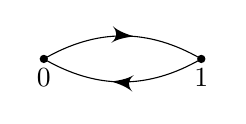
\begin{tikzpicture}
      \node [circ] at (0, 0) {};
      \node [circ] at (2, 0) {};
      \node [below] at (0, 0) {$0$};
      \node [below] at (2, 0) {$1$};

      \draw (0, 0) edge [bend left, ->-=0.57] (2, 0); %insert node saying $1$
      \draw (2, 0) edge [bend left, ->-=0.57] (0, 0);

    \end{tikzpicture}
  \end{center}
\end{eg}

\begin{eg}
  Take $\Gamma = S_3$ and $S = \{(1\; 2), (1\; 2\; 3)\}$. The Cayley graph is
  \begin{center}
    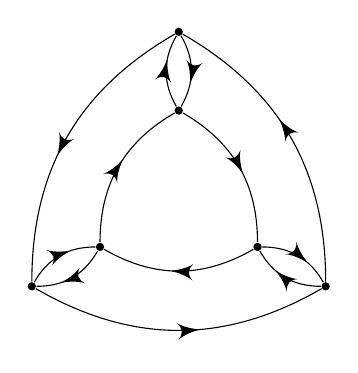
\begin{tikzpicture}
      \node [circ] (L) at (0, 0) {};
      \node [circ] (R) at (2, 0) {};
      \node [circ] (T) at (1, 1.732) {};
      \node [circ] (LL) at (-0.866, -0.5) {};
      \node [circ] (RR) at (2.866, -0.5) {};
      \node [circ] (TT) at (1, 2.732) {}; % this is wrong

%      \node [below] at (L) {$1$};
%      \node at (R) {$(3\; 2\; 1)$};
%      \node at (T) {$(1\; 2\; 3)$};
%      \node at (LL) {$(1\; 2)$};

      \draw (L) edge [bend left, ->-=0.55] (T);
      \draw (T) edge [bend left, ->-=0.55] (R);
      \draw (R) edge [bend left, ->-=0.55] (L);

      \draw (TT) edge [bend right, ->-=0.57] (LL);
      \draw (LL) edge [bend right, ->-=0.57] (RR);
      \draw (RR) edge [bend right, ->-=0.57] (TT);

      \draw (T) edge [bend left, ->-=0.66] (TT);
      \draw (TT) edge [bend left, ->-=0.66] (T);

      \draw (R) edge [bend left, ->-=0.66] (RR);
      \draw (RR) edge [bend left, ->-=0.66] (R);

      \draw (L) edge [bend left, ->-=0.66] (LL);
      \draw (LL) edge [bend left, ->-=0.66] (L);
    \end{tikzpicture}
  \end{center}
\end{eg}

\begin{eg}
  Take $\Gamma = \Z$, and $S = \{1\}$. Then the Cayley graph looks like
  \begin{center}
    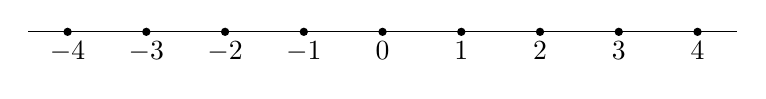
\begin{tikzpicture}
      \foreach \x in {-4,-3,-2,-1,0,1,2,3,4} {
        \node [circ] at (\x, 0) {};
        \node [below] at (\x, 0) {$\x$};
      }
      \draw (-4.5, 0) -- (4.5, 0);
    \end{tikzpicture}
  \end{center}
\end{eg}
\begin{eg}
  Take $\Gamma = \Z$ and $S = \{2, 3\}$. Then the Cayley graph looks like
  \begin{center}
    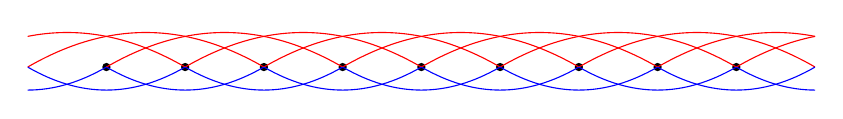
\begin{tikzpicture}
      \clip (-5, -0.3) rectangle (5, 0.5);
      \foreach \x in {-4,-3,-2,-1,0,1,2,3,4} {
        \node [circ] at (\x, 0) {};
      }
      \foreach \x in {-6,-5,-4,-3,-2,-1,0,1,2,3,4} {
        \draw [red] (\x, 0) edge [bend left] +(3, 0);
        \draw [blue] (\x, 0) edge [bend right] +(2, 0);
      }
    \end{tikzpicture}
  \end{center}
\end{eg}
Now this seems quite complicated. It's still the same group $\Gamma = \Z$, but with a different choice of generating set, it looks very different. It seems like what we do depends heavily on the choice of the generating set.

\begin{eg}
  If $\Gamma = \Z^2$ and $S = \{(1, 0), (0, 1)\}$, then the Cayley graph is a grid
  \begin{center}
    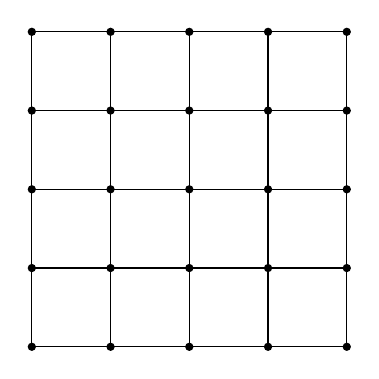
\begin{tikzpicture}
      \foreach \x in {-2,-1,0,1,2} {
        \foreach \y in {-2,-1,0,1,2} {
          \node [circ] at (\x, \y) {};
        }
      }
      \draw [step=1] (-2, -2) grid (2, 2);
    \end{tikzpicture}
  \end{center}
\end{eg}

\begin{eg}
  If $\Gamma = F_2 = \bra a, b\ket$, $S = \{a, b\}$, then the Cayley graph looks like
  \begin{center}
    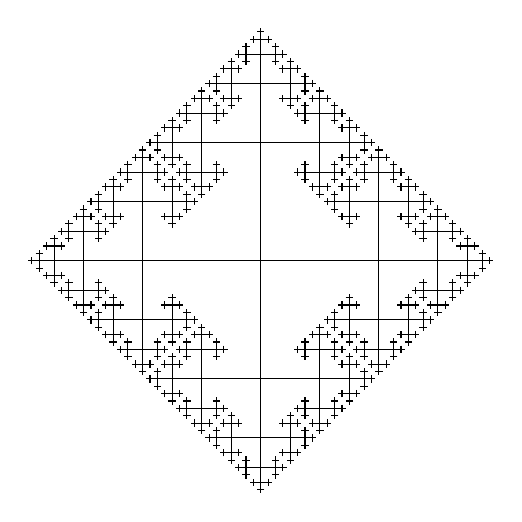
\begin{tikzpicture}[scale=0.5]
      \draw (-3, 0) -- (3, 0);
      \draw (0, -3) -- (0, 3);
      \foreach \x/\y/\rot in {3/0/0, 0/3/90, -3/0/180, 0/-3/270} {
        \begin{scope}[shift={(\x, \y)}, scale=0.5, rotate=\rot]
          \draw (0, 0) -- (3, 0);
          \draw (0, 3) -- (0, -3);
          \foreach \x/\y/\rot in {3/0/0, 0/3/90, 0/-3/270} {
            \begin{scope}[shift={(\x, \y)}, scale=0.5, rotate=\rot]
              \draw (0, 0) -- (3, 0);
              \draw (0, 3) -- (0, -3);
              \foreach \x/\y/\rot in {3/0/0, 0/3/90, 0/-3/270} {
                \begin{scope}[shift={(\x, \y)}, scale=0.5, rotate=\rot]
                  \draw (0, 0) -- (3, 0);
                  \draw (0, 3) -- (0, -3);
                  \foreach \x/\y/\rot in {3/0/0, 0/3/90, 0/-3/270} {
                    \begin{scope}[shift={(\x, \y)}, scale=0.5, rotate=\rot]
                      \draw (0, 0) -- (3, 0);
                      \draw (0, 3) -- (0, -3);
                      \foreach \x/\y/\rot in {3/0/0, 0/3/90, 0/-3/270} {
                        \begin{scope}[shift={(\x, \y)}, scale=0.5, rotate=\rot]
                          \draw (0, 0) -- (3, 0);
                          \draw (0, 3) -- (0, -3);
                        \end{scope}
                      }
                    \end{scope}
                  }
                \end{scope}
              }
            \end{scope}
          }
        \end{scope}
      }
    \end{tikzpicture}
  \end{center}
\end{eg}
If one has done algebraic topology, then one might recognize this as the universal cover of a space. This is not a coincidence, and we will talk about this later.

We now return to the problem we noticed previously. The Cayley graph depends a lot on the generating set chosen, but we want to study the graph without picking a generating set.

What we observe is that while the two Cayley graphs of $\Z$ we drew seem quite different, if we looked at them from $100$ meters away, they look quite similar --- they both look like a long, thin line. This is the idea we are trying to formalize.

\begin{defi}[Quasi-isometry]\index{quasi-isometry}\index{quasi-isometric embedding}
  Let $\lambda \geq 1$ and $c \geq 0$. A function between metric spaces $f: X \to Y$ is a \emph{$(\lambda, c)$-quasi-isometric embedding} if for all $x_1, x_2 \in X$
  \[
    \frac{1}{\lambda} d_X(x_1, x_2) - c \leq d_Y(f(x_1), f(x_2)) \leq \lambda d_X(x,_1, x_2) + c
  \]
  If, in addition, there is a $C$ such that for all $y \in Y$, there exists $x \in X$ such that $d_Y(y, f(x)) \leq C$, we say $f$ is a \emph{quasi-isometry}, and $X$ is \term{quasi-isometric} to $Y$. We write $X\qi Y$.
\end{defi}
We can think of the first condition as saying we are \term{quasi-injective}, and the second as saying we are \term{quasi-surjective}.

The right way to think about the definition is that the $c$ says we don't care about what happens at scales less than $c$, and the $\lambda$ is saying we allow ourselves to stretch distances. Note that if we take $c = 0$, then this is just the notion of a bi-Lipschitz map. But in general, we don't even require $f$ to be continuous, since continuity is a rather fine-grained property.

\begin{ex}
  Check that $ X\qi Y$ is an equivalence relation.
\end{ex}
This is not immediately obvious, because there is no inverse to $f$. In fact, we need the axiom of choice to prove this result.

\begin{eg}
  Any bounded metric spaces is quasi-isometric to a point. In particular, if $\Gamma$ is finite, then $(\Gamma, d_S) \qi 1$.
\end{eg}
For this reason, this is not a great point of view for studying finite groups. On the other hand, for infinite groups, this is really useful.

\begin{eg}
  For any $\Gamma$ and $S$, the inclusion $(\Gamma, \Gamma_S)\hookrightarrow (\Cay_S(\Gamma), d_S)$ is a quasi-isometry (take $\lambda = 1, c = 0, C = \frac{1}{2}$).
\end{eg}

Of course, the important result is that any two word metrics on the same group are quasi-isomorphic.
\begin{thm}
  For any two finite generating sets $S, S'$ of a group $\Gamma$, the identity map $(\Gamma, d_S) \to (\Gamma, d_{S'})$ is a quasi-isometry.
\end{thm}

\begin{proof}
  Pick
  \[
    \lambda = \max_{s \in S} \ell_{S'}(s),\quad \lambda' \max_{s \in S'} \ell_{S}(s),
  \]
  We then see
  \[
    \ell_S(\gamma) \leq \lambda' \ell_{S'}(\gamma), \quad \ell_{S'}(\gamma) \leq \lambda \ell_s(\gamma). % check
  \]
  for all $\gamma \in \Gamma$. Then the claim follows.
\end{proof}
So as long as we are willing to work up to quasi-isometry, we have a canonically defined geometric object associated to each finitely-generated group.

Our next objective is to be able to state and prove the Schwarz--Milnor lemma. This is an important theorem in geometric group theory, saying that if a group $\Gamma$ acts ``nicely'' on a metric space $X$, then $\Gamma$ must be finitely generated, and in fact $(\Gamma, d_s)$ is quasi-isomorphic to $X$. This allows us to produce some rather concrete geometric realizations of $(\Gamma, d_s)$, as we will see in examples.

In order to do that, we must write down a bunch of definitions.

\begin{defi}[Geodesic]\index{geodesic}
  Let $X$ be a metric space. A \emph{geodesic} in $X$ is an isometric embedding of a closed interval $\gamma: [a, b] \to X$.
\end{defi}
This is not exactly the same as the notion in differential geometry. For example, if we have a sphere and two non-antipodal points on the sphere, then there are many geodesics connecting them in the differential geometry sense, but only the shortest one is a geodesic in our sense. To recover the differential geometry notion, we need to insert the words ``locally'' somewhere, but we shall not care about that.

\begin{defi}[Geodesic metric space]\index{geodesic metric space}\index{metric space!geodesic}
  A metric space $X$ is called \emph{geodesic} if every pair of points $x, y \in X$ is joined by a geodesic denoted by $[x, y]$.
\end{defi}
Note that the notation $[x, y]$ is not entirely honest, since there may be many geodesics joining two points.

\begin{defi}[Proper metric space]\index{proper metric space}
  A metric space is \emph{proper} if closed balls in $X$ are compact.
\end{defi}

\begin{eg}
  If $\Gamma = \langle S\rangle$, then $\Cay_S(\Gamma)$ is geodesic. If $S$ is finite, then $\Cay_S(\Gamma)$ is proper.
\end{eg}

\begin{eg}
  Let $M$ be a connected Riemannian manifold. Then there is a metric on $M$ defined by
  \[
    d(x, y) = \inf_{\alpha: x \to y} \length(\alpha),
  \]
  where we take the infimum over all smooth paths from $x$ to $y$.

  The \term{Hopf--Rinow theorem} says if $M$ is complete (as a metric space), then the metric is proper and geodesic. This is great, because completeness is in some sense a local property, but ``proper'' and ``geodesic'' are global properties.
\end{eg}

We need two more definitions, before we can state the Schwarz--Milnor lemma.
\begin{defi}[Proper discontinuous action]\index{proper discontinuous action}
  An action $\Gamma$ on a topological space $X$ is \emph{proper discontinuous} if for every compact set $K$,
  \[
    \{g \in \Gamma: gK \cap K \not= \emptyset\}
  \]
  is finite.
\end{defi}

\begin{defi}[Cocompact action]\index{cocompact action}
  An action $\Gamma$ on a topological space $X$ is \emph{cocompact} if the quotient $\Gamma \setminus X$ is compact.
\end{defi}

\begin{lemma}[Schwarz--Milnor lemma]
  Let $X$ be a proper geodesic metric space, and let $\Gamma$ act properly discontinuously, cocompactly on $X$ by isometries. Then
  \begin{enumerate}
    \item $\Gamma$ is finitely-generated.
    \item For any $x_0 \in X$, the orbit map
      \begin{align*}
        \Gamma &\to X\\
        \gamma &\mapsto \gamma x_0
      \end{align*}
      is a quasi-isometry $(\Gamma, d_s) \qi (X, d)$.
  \end{enumerate}
\end{lemma}
An easy application is that $\Gamma$ acting on its Caylay graph satisfies these conditions. So this reproduces our previous observation that a group is quasi-isometric to its Cayley graph. More interesting examples involve manifolds.

\begin{eg}
  Let $M$ be a closed (i.e.\ compact without boundary), connected Riemannian manifold. Then the universal cover $\tilde{M}$ is also a complete, connected, Riemannian manifold. By the Hopf--Rinow theorem, this is proper and geodesic.

  Since the metric of $\tilde{M}$ is pulled back from $M$, we know $\pi_1(M)$ acts on $\tilde{M}$ by isometries. Therefore by the Schwarz--Milnor lemma, we know
  \[
     \pi_1(M) \qi \tilde{M}.
  \]
\end{eg}
\begin{eg}
  The universal cover of the torus $S^1 \times S^1$ is $\R^2$, and the fundamental group is $\Z^2$. So we know $\Z^2 \qi \R^2$, which is not surprising.
\end{eg}

\begin{eg}
  Let $M = \Sigma_2$, the surface of genus $2$.
  \begin{center}
    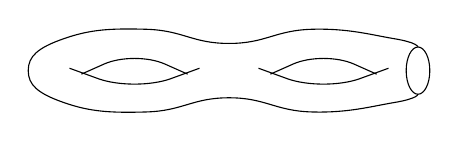
\begin{tikzpicture}[scale=1.5]
      \draw plot [smooth, tension=0.8] coordinates {(1.6, 0.2) (1.4, 0.27) (0.7, 0.35) (0, 0.23) (-0.7, 0.35) (-1.4, 0.27) (-1.7, 0) (-1.4, -0.27) (-0.7, -0.35) (0, -0.23) (0.7, -0.35) (1.4, -0.27) (1.6, -0.2)};
      \draw (1.6, 0) ellipse (0.1 and 0.2);

      \foreach \x in {0.8, -0.8}{
        \begin{scope}[shift={(\x, -0.03)}]
          \path[rounded corners=12pt] (-0.45, 0)--(0, 0.2)--(0.45, 0) (-0.45, 0)--(0, -0.28)--(0.45, 0);
          \draw[rounded corners=14pt] (-0.55, 0.05)--(0, -.15)--(0.55, 0.05);
          \draw[rounded corners=12pt] (-0.45, 0)--(0, 0.2)--(0.45, 0);
        \end{scope}
      }
    \end{tikzpicture}
  \end{center}
  We then have
  \[
    \pi_1 \Sigma_2 \cong \langle a_1, b_1, a_2, b_2 \mid [a_1, b_1][a_2, b_2]\rangle.
  \]
  On the other hand, the universal cover can be thought of as the hyperbolic plane $\H^2$, as we saw in IB Geometry. % insert picture!!

  So it follows that
  \[
    \pi_1 \Sigma_2 \qi \H^2.
  \]
\end{eg}
This gives us some concrete hold on what the group $\pi_1 \Sigma_2$ is like, since people have been thinking about the hyperbolic plane for centuries.

After all those applications, we can start to write down a proof.
\begin{proof}[Proof of Schwarz--Milnor lemma]
  Let $\bar{B} = \bar{B}(x, R)$ be such that $\Gamma \bar{B} = X$. This is possible since the quotient is compact.

  Let $S = \{\gamma \in \Gamma: \gamma \bar{B} \cap \bar{B} \not=\emptyset\}$. By proper discontinuity, this set is finite.

  We let
  \[
    r = \inf_{\gamma' \not \in S} d(\bar{B}, \gamma' \bar{B}).
  \]
  If we think about it, we see that in fact $r$ is the \emph{minimum} of this set, and in particular $r > 0$.

  Finally, let
  \[
    \lambda = \max_{s \in S} d(x_0, s x_0).
  \]
  We will show that $S$ generates $\Gamma$, and use the word metric given by $S$ to show that $\Gamma$ is quasi-isometric to $X$.

  We first show that $\Gamma = \langle S\rangle$. We let $\gamma \in \Gamma$ be arbitrary.

  Let $[x_0, \gamma x_0]$ be a geodesic from $x_0$ to $\gamma x_0$. Let $\ell$ be such that
  \[
    (\ell - 1)r \leq d(x_0, \gamma x_0) < \ell r.
  \]
  Then we can divide the geodesic into $\ell$ pieces of length about $r$. We can choose $x_1, \ldots x_{\ell - 1}, x_\ell = \gamma x_0$ such that $d(x_{i - 1}, x_i) < r$.

  By assumption, we can pick $\gamma_i \in \Gamma$ such that $x_i \in \gamma_i \bar{B}$, and further we pick $\gamma_\ell = \gamma$, $\gamma_0 = e$. Now for each $i$, we know
  \[
    d(\bar{B}, \gamma_{i -1 }^{-1} \gamma_i \bar{B}) = d(\gamma_{i - 1} \bar{B}, \gamma_i \bar{B}) \leq d(x_{i - 1}, x_i) < r.
  \]
  So it follows that $\gamma_{i - 1}^{-1} \gamma_i \in S$. So we have
  \[
    \gamma = \gamma_\ell = (\gamma_0^{-1} \gamma_1) (\gamma_1^{-1}\gamma_2) \cdots (\gamma_{\ell - 1}^{-1}\gamma_\ell) \in \langle S\rangle.
  \]
  This proves $\Gamma = \langle S \rangle$.

  To prove the second part, we simply note that
  \[
    r\ell - r \leq d (x_0 \gamma x_0).
  \]
  We also saw that $\ell$ is an upper bound for the word length of $\gamma$ under $S$. So we have
  \[
    r \ell_s(\gamma) - r \leq d(x_0, \gamma x_0).
  \]
  On the other hand, by definition of $\lambda$, we have
  \[
    d(x_0, \gamma x_0) \leq \lambda \ell_s(\gamma).
  \]
  So the orbit map is an orbit-embedding, and quasi-surjectivity follows from cocompactness.
\end{proof}

If we want to understand a group, then a reasonable strategy now would be to come up with a well-understood (proper geodesic) space for $\Gamma$ to act (proper discontinuously, cocompactly) on, and see what we can tell from this quasi-isometry. There is no general algorithm for doing so, but we shall see that for certain groups, there are some ``obvious'' good choices to make.

\subsection{Free groups}
Let's begin by understanding the free group. In some sense, they are the ``simplest'' groups, but they also contain some rich structure. Roughly speaking, a free group on a set $S$ is a group that is ``freely'' generated by $S$. This freeness is made precise by the following universal property.

\begin{defi}[Free group]\index{free group}\index{$F(S)$}
  Let $S$ be a (usually finite) set. A group $F(S)$ with a map $S \to F(S)$ is called the \emph{free group on $S$} if it satisfies the following universal property: for any set map $S \to G$, there is a unique group homomorphism $F(S) \to G$ such that the following diagram commutes:
  \[
    \begin{tikzcd}
      S \ar[r] \ar[rd, dashed] & F(S) \ar[d]\\
      & G
    \end{tikzcd}.
  \]
  Usually, if $|S| = r$, we just write $F(S) = F_r$.\index{$F_r$}
\end{defi}

In fancy category-theoretic language, this says the functor $F: \mathbf{Sets} \to \mathbf{Grps}$ is left adjoint to the forgetful functor $U: \mathbf{Grps} \to \mathbf{Sets}$.

This definition is good for some things, but not good for others. One thing it does well is it makes it clear that $F(S)$ is unique up to isomorphism if it exists. However, it is not immediately clear that $F(S)$ exists! (unless one applies the adjoint functor theorem)

Thus, we must concretely construct a group satisfying this property, and this construction is often useful if we actually want to work with the set.

For concreteness, suppose $S = \{a_1, \ldots, a_r\}$ is a finite set. We consider a graph
\[
  X_r =
  \begin{tikzpicture}[eqpic, scale=3]
    \node [circ] {};
    \foreach \r in {-130,-65,0,65,130} {
      \draw [rotate=\r] (0, 0) edge [out=-30, in=30, looseness=2, loop] (0, 0);
    }

    \node at (-0.2, 0.03) {$\vdots$};
  \end{tikzpicture}
\]
where there are $r$ ``petals''. This is known as the \term{rose with $r$ petals}.

We claim that its fundamental group is $F(S)$. To see this, we have to understand the universal cover $\tilde{X}_r$ of $X_r$. We know $\tilde{X}_r$ is a simply connected graph, so it is a tree. Moreover, since it is a covering space of $X_r$, it is regular with degree $2r$ on each vertex.

If $r = 2$, then this is our good old picture % label edges as a_1 (horizontal) and a_2 (vertical), and label basepoint as *
\begin{center}
  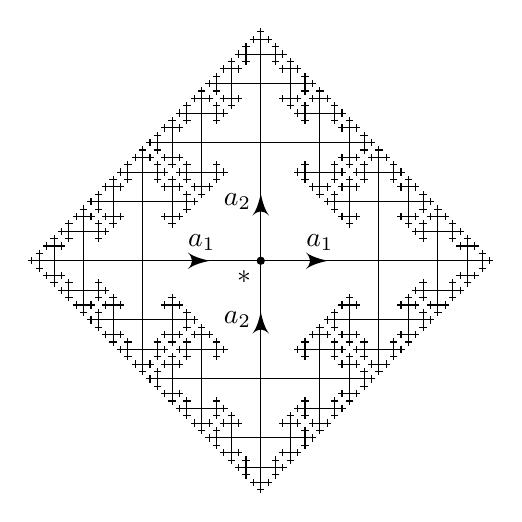
\begin{tikzpicture}[scale=0.5]
    \draw (-3, 0) -- (3, 0);
    \draw (0, -3) -- (0, 3);
    \foreach \x/\y/\rot in {3/0/0, 0/3/90, -3/0/180, 0/-3/270} {
      \begin{scope}[shift={(\x, \y)}, scale=0.5, rotate=\rot]
        \draw (0, 0) -- (3, 0);
        \draw (0, 3) -- (0, -3);
        \foreach \x/\y/\rot in {3/0/0, 0/3/90, 0/-3/270} {
          \begin{scope}[shift={(\x, \y)}, scale=0.5, rotate=\rot]
            \draw (0, 0) -- (3, 0);
            \draw (0, 3) -- (0, -3);
            \foreach \x/\y/\rot in {3/0/0, 0/3/90, 0/-3/270} {
              \begin{scope}[shift={(\x, \y)}, scale=0.5, rotate=\rot]
                \draw (0, 0) -- (3, 0);
                \draw (0, 3) -- (0, -3);
                \foreach \x/\y/\rot in {3/0/0, 0/3/90, 0/-3/270} {
                  \begin{scope}[shift={(\x, \y)}, scale=0.5, rotate=\rot]
                    \draw (0, 0) -- (3, 0);
                    \draw (0, 3) -- (0, -3);
                    \foreach \x/\y/\rot in {3/0/0, 0/3/90, 0/-3/270} {
                      \begin{scope}[shift={(\x, \y)}, scale=0.5, rotate=\rot]
                        \draw (0, 0) -- (3, 0);
                        \draw (0, 3) -- (0, -3);
                      \end{scope}
                    }
                  \end{scope}
                }
              \end{scope}
            }
          \end{scope}
        }
      \end{scope}
    }
    \node [circ] {};
    \node [anchor = north east] {$*$};
    \draw [->] (1.7, 0) -- (1.71, 0);
    \node [above] at (1.5, 0) {$a_1$};
    \draw [->] (-1.3, 0) -- (-1.29, 0);
    \node [above] at (-1.5, 0) {$a_1$};

    \draw [->] (0, 1.7) -- (0, 1.71);
    \node [left] at (0, 1.5) {$a_2$};
    \draw [->] (0, -1.3) -- (0, -1.29);
    \node [left] at (0, -1.5) {$a_2$};

  \end{tikzpicture}
\end{center}

We can use this to understand the fundamental group $\pi_1(X_r)$. The elements on $\pi_1 (X_r)$ are homotopy classes [$\gamma$] of based loops in $X_r$. Using the homotopy lifting lemma, this map can be lifted to a path $\tilde{\gamma}$ in the universal cover starting at $*$.
\begin{center}
  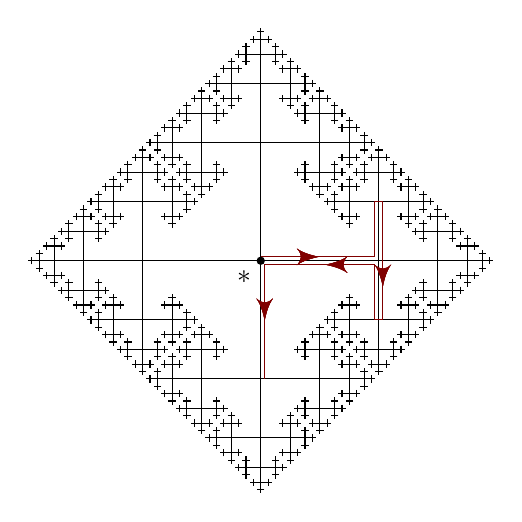
\begin{tikzpicture}[scale=0.5]
    \draw (-3, 0) -- (3, 0);
    \draw (0, -3) -- (0, 3);
    \foreach \x/\y/\rot in {3/0/0, 0/3/90, -3/0/180, 0/-3/270} {
      \begin{scope}[shift={(\x, \y)}, scale=0.5, rotate=\rot]
        \draw (0, 0) -- (3, 0);
        \draw (0, 3) -- (0, -3);
        \foreach \x/\y/\rot in {3/0/0, 0/3/90, 0/-3/270} {
          \begin{scope}[shift={(\x, \y)}, scale=0.5, rotate=\rot]
            \draw (0, 0) -- (3, 0);
            \draw (0, 3) -- (0, -3);
            \foreach \x/\y/\rot in {3/0/0, 0/3/90, 0/-3/270} {
              \begin{scope}[shift={(\x, \y)}, scale=0.5, rotate=\rot]
                \draw (0, 0) -- (3, 0);
                \draw (0, 3) -- (0, -3);
                \foreach \x/\y/\rot in {3/0/0, 0/3/90, 0/-3/270} {
                  \begin{scope}[shift={(\x, \y)}, scale=0.5, rotate=\rot]
                    \draw (0, 0) -- (3, 0);
                    \draw (0, 3) -- (0, -3);
                    \foreach \x/\y/\rot in {3/0/0, 0/3/90, 0/-3/270} {
                      \begin{scope}[shift={(\x, \y)}, scale=0.5, rotate=\rot]
                        \draw (0, 0) -- (3, 0);
                        \draw (0, 3) -- (0, -3);
                      \end{scope}
                    }
                  \end{scope}
                }
              \end{scope}
            }
          \end{scope}
        }
      \end{scope}
    }
    \node [circ] {};
    \node [anchor = north east] {$*$};
    \draw [mred, ->-=0.1, ->-=0.45, ->-=0.7, ->-=0.9] (0, 0.1) -- (2.9, 0.1) -- (2.9, 1.5) -- (3.1, 1.5) -- (3.1, -1.5) -- (2.9, -1.5) -- (2.9, -0.1) -- (0.1, -0.1) -- (0.1, -3);
  \end{tikzpicture}
\end{center}
Since this is a loop, we know it ends at another vertex. Because $\tilde{X}_r$ is a tree, we may homotope $\tilde{\gamma}$ rel endpoints to the unique embedded path from $*$ to the endpoint of $\tilde{\gamma}$. We can push this homotopy down to $X_r$ to get a homotopy of $\gamma$. We can see that $\gamma$ is of the following form:
\[
  \gamma = a_{i_1}^{\pm 1} a_{i_2}^{\pm 1} a_{i_3}^{\pm 1}\cdots a_{i_n}^{\pm 1}.
\]
Moreover, since $\tilde{\gamma}$ is now embedded, we know $\gamma$ is reduced, i.e.\ we never see anything looking like $a_i^{\pm 1} a_i^{\mp 1}$. Importantly, this form is unique. There is only one way to write $\gamma$ in this form. This gives us a \term{normal form theorem} for elements in $\pi_1(X_r)$ --- every element in $\pi_1(X_r)$ is represented by a unique reduced word in the generators. So if we have two elements in $\pi_1(X_r)$ expressed as products of generators and their inverses, then to determine if they are equal, we can individually reduce the two words in any way we like, and check if the result is the same.

\begin{eg}
  Take the case $\pi_1 X_2 = \langle a, b\rangle$. We might be given a word
  \[
    a^3 a^{-2} b^{-2} b^3 a^5 a^{-3} a^{-3} b^{-1}.
  \]
  We can reduce this to
  \[
    a ba^{-1}b^{-1}.
  \]
  In particular, since this is not the identity, we know the original path was not null-homotopic.
\end{eg}

As a consequence of this, we see that
\begin{cor}
  $\pi_1(X_r)$ has the universal property of $F(S)$, with $S = \{a_1, \ldots, a_r\}$. So $\pi_1(X_r) \cong F_r$.
\end{cor}

\begin{proof}
  Given any map $f: S \to G$, define $\tilde{f}: F(S) \to G$ by
  \[
    \tilde{f}(a_{i_1}^{\pm 1}\cdots a_{i_n}^{\pm 1}) = \tilde{f}(a_i)^{\pm 1} \cdots \tilde{f}(a_{i_n})^{\pm 1}
  \]
  for any reduced word $a_{i_1}^{\pm 1} \cdots a_{i_n}^{\pm 1}$. This is easily seen to be well-defined and is the unique map making the diagram commute.
\end{proof}

\subsection{Finitely-presented groups}
Now if a group $\Gamma$ is generated by $S$, then we have a surjective homomorphism $F(S) \to \Gamma$. Let $K = \ker \eta$. Then
\[
  \Gamma \cong \frac{F(S)}{K}.
\]
Since we understand $F(S)$ quite explicitly, it would be nice if we have a solid gasp on $K$ as well. If $R$ normally generates $K$, so that $K = \bra\bra R\ket\ket$, then we say that $\bra S \mid R \ket$ is a \term{presentation} for $\Gamma$. We will often write that
\[
  \Gamma \cong \langle S \mid R \rangle.
\]
\begin{eg}
  \[
    \Z^2 = \langle a, b\mid aba^{-1}b^{-1}\rangle
  \]
\end{eg}

\begin{defi}[Finitely-presented group]\index{finitely-presented group}\index{finitely-presentable group}
  A \emph{finitely-presentable group} is a group $\Gamma$ such that there are finite $S$ and $R$ such that $\Gamma \cong \bra S \mid R\ket$.

  A \emph{finitely-presented group} is a group $\Gamma$ equipped $S$ and $R$ such that $\Gamma \cong \bra S \mid R \ket$.
\end{defi}

Presentations give us ways to geometrically understand a group. Given a presentation $\mathcal{P} = \langle S \mid R \rangle$, we can construct space \term{$X_\mathcal{P}$} such that $\pi_1 X_\mathcal{P} \cong \bra S \mid R\ket$

To do so, we first construct a rose with $|S|$ many petals, each labeled by an element of $S$. For each $r \in R$, glue a disk onto the rose along the path specified by $r$. The \term{Seifert--van Kampen theorem} then tells us $\pi_1 X_{\mathcal{P}} \cong \Gamma$.

\begin{eg}
  We take the presentation $\Z^2 \cong \bra a, b \mid aba^{-1}b^{-1}\ket$. If we think hard enough (or a bit), we see this construction gives the torus.
\end{eg}

Conversely, if we are given a connected cell complex $X$, we can obtain a presentation of the fundamental group. This is easy if the cell complex has a single $0$-cell. If it has multiple $0$-cells, then we choose a maximal tree in $X^{(1)}$, and the edges $S = \{a_i\}$ not in the maximal tree define a generating set for $\pi_1 X^{(1)}$. The attaching maps of the $2$-cells in $X$ define elements $R = \{r_j\}$ of $\pi_1 X^{(1)}$, and these data define a presentation $\mathcal{P}_X = \bra S \mid R\ket$ for $\pi_1 X$.

This is not canonical, since we have to pick a maximal tree, but let's not worry too much about that. The point of maximal trees is to get around the problem that we might have more than one vertex.

\begin{ex}
  If $X$ has one vertex, then $\Cay_S \pi_1 X = \tilde{X}^{(1)}$.
\end{ex}

\subsection{The word problem}
Before we try to understand the word problem, let's give some historical perspectives. Long time ago, Poincar\'e was interested in characterizing the $3$-sphere. His first conjecture was that if a closed $3$-manifold $M$ had $H_*(M) \cong H_*(S^3)$, then $M \cong S^3$. Poincar\'e thought very hard about the problem, and came up with a counterexample. The counterexample is known as the \term{Poincar\'e homology sphere}\index{homology sphere}. This is a manifold $P^3$ with
\[
  H_*(P) \cong H_*(S^3),
\]
but it turns out there is a surjection $\pi_1(P^3) \to A_5$. In particular, $P^3$ is not homeomorphic to a sphere.

So he made a second conjecture, that if $M$ is a compact manifold with $\pi_1M \cong 1$, then $M \cong S^3$. Note that the condition already implies $H_*(M) \cong H_*(S^3)$ by Hurewicz theorem and Poincar\'e duality. This is known as the Poincar\'e conjecture, which was proved in 2002 by Perelman.

But there is more to say about Poincar\'e's initial conjecture. Some time later, Max Dehn constructed an \emph{infinite family} of 3d homology spheres. In order to prove that he genuinely had infinitely many distinct homology spheres, he had to show that his homology spheres had different fundamental groups. He did manage to write down the presentations of the fundamental groups, and so what was left to do is to distinguish whether the presentations actually presented the same group.

To make sense of this statement, we must have some way to distinguish between the homology spheres. To do so, he managed to write down the presentation of the fundamental group of his homology spheres, and he had to figure out if those groups are genuinely the same.

For our purposes, perhaps we should be slightly less ambitious. Suppose we are given a presentation $\bra S \mid R\ket$ of a finitely-presented group $\Gamma$. Define the set of alphabets
\[
  S^{\pm} = S \amalg S^{-1} = \{ s, s^{-1}: s \in S\},
\]
and let $S^*$ be the set of all finite words in $S^{\pm}$. Then the fundamental question is, given a word $w \in S^*$, when does it represent the identity element $1 \in \Gamma$. Ideally, we would want an \emph{algorithm} that determines whether this is the case.

\begin{eg}
  Recall that in the free group $F(S) = \bra S \mid \emptyset\ket$, we had a normal form theorem, namely that every element in $\Gamma$ can be written \emph{uniquely} as a product of generator (and inverses) such that there aren't any occurrences of $ss^{-1}$ or $s^{-1}s$. This gives a way of determining whether a given word $w \in S^*$ represents the identity. We perform \term{elementary reductions}, removing every occurrence of $ss^{-1}$ or $s^{-1}s$. Since each such procedure reduces the length of the word, this eventually stops, and we would end up with a \term{reduced word}. If this reduced word is empty, then $w$ reduces the identity. If it is non-empty, $w$ does not.
\end{eg}
Thus, we have a complete solution to the word problem for free groups, and moreover the algorithm is something we can practically implement.

For a general finitely-presented group, this is more difficult. We can first reformulate our problem. The presentation $\Gamma = \bra S \mid R \ker$ gives us a map $F(S) \to \Gamma$, sending $s$ to $s$. Each word gives us an element in $F(S)$, and thus we can reformulate our problem as identifying the elements in the kernel of this map.

\begin{lemma}
  Let $\Gamma = \bra S \mid R\ket$. Then the elements of $\ker \{F(S) \to \Gamma\}$ are precisely those of the form
  \[
    \prod_{i = 1}^d g_i r_i^{\pm 1} g_i^{-1},
  \]
  where $g_i \in F(S)$ and $r_i \in R$.
\end{lemma}

\begin{proof}
  We know that $\ker \{F(S) \to \Gamma\} = \bra \bra R\ket \ket$, and the set described above is exactly $\bra \bra R\ket \ket$, noting that $gxyg^{-1} = (gxg^{-1})(gyg^{-1})$.
\end{proof}

This tells us the set of elements in $S^*$ that represent the identity is \term{recursively enumerable}, i.e.\ there is an algorithm that lists out all words that represent the identity. However, this is not very helpful when we want to identify whether a word represents the identity. If it does, then our algorithm will eventually tell us it is (maybe after 3 trillion years), but if it doesn't, the program will just run forever, and we will never know that it doesn't represent the identity.

It turns out the answer to this question has some geometric interpretations. Let's first look at the example.
\begin{eg}
  Let $\Gamma = \Z^2 \cong \bra a, b \mid [a, b]\ket$. Consider the word
  \[
    w = a^n b^n a^{-n} b^{-n}
  \]
  We see that this represents our identity element. But how long would it take for our algorithm to figure this fact out? Equivalently, what $d$ do we need to pick so that $w$ is of the form
  \[
    \prod_{i = 1}^d g_i r_i^{\pm 1} g_i^{-1}?
  \]
  We can draw a picture. Our element $[a, b]$ looks like
  \begin{center}
    \begin{tikzpicture}
      \draw (0, 0) rectangle (1, 1);
      \node [right] at (1, 0.5) {$b$};
      \node [left] at (0, 0.5) {$b$};
      \node [below] at (0.5, 0) {$a$};
      \node [above] at (0.5, 1) {$a$};
    \end{tikzpicture}
  \end{center}
  If, say, $n = 2$, then $w$ is given by
  \begin{center}
    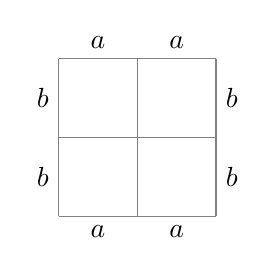
\begin{tikzpicture}
      \draw [step=1, gray] (0, 0) grid (2, 2);
      \foreach \x in {0.5,1.5} {
         \node [below] at (\x, 0) {$a$};
         \node [above] at (\x, 2) {$a$};
         \node [right] at (2, \x) {$b$};
         \node [left] at (0, \x) {$b$};
      }
    \end{tikzpicture}
  \end{center}
  If we think about it hard, then we see that what we need to do is to find out how to fill in this big square with the small squares, and we need $4$ squares. Indeed, we can read off the sequence
  \[
    w = [a, b] \cdot (b [a, b] b^{-1}) \cdot (b^2 a b^{-1} [a, b] ba^{-1} b^{-2}) \cdot (b^2 a^2 b^{-1}a^{-1}b^{-1}[a, b]baba^{-2}b^{-2}),
  \]
  which corresponds to filling in the square one by one as follows:
  \begin{center}
    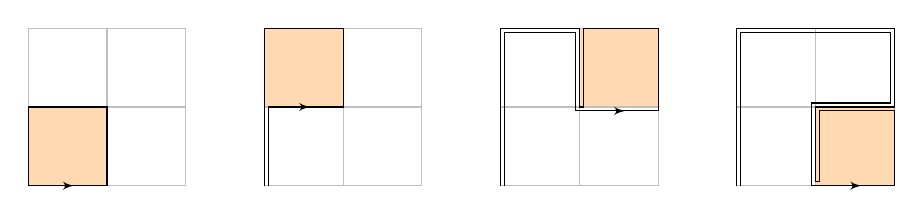
\begin{tikzpicture}
      \fill [opacity=0.3, morange] (0, 0) rectangle +(1, 1);
      \draw [step=1, gray!50!white] (0, 0) grid (2, 2);
      \draw (0, 0) rectangle (1, 1);
      \draw [-latex'] (0.58, 0) -- +(0.001, 0);

      \begin{scope}[shift={(3, 0)}]
        \fill [opacity=0.3, morange] (0, 1) rectangle +(1, 1);
        \draw [step=1, gray!50!white] (0, 0) grid (2, 2);
        \draw (0, 0) -- (0, 2) -- (1, 2) -- (1, 1) -- (0.05, 1) -- (0.05, 0);

        \draw [-latex'] (0.58, 1) -- +(0.001, 0);
      \end{scope}
      \begin{scope}[shift={(6, 0)}]
        \fill [opacity=0.3, morange] (1, 1) rectangle +(1, 1);
        \draw [step=1, gray!50!white] (0, 0) grid (2, 2);
        \draw (0, 0) -- (0, 2) -- (1, 2) -- (1, 1) -- (1.05, 1) -- (1.05, 2) -- (2, 2) -- (2, 0.95) -- (0.95, 0.95) -- (0.95, 1.95) -- (0.05, 1.95) -- (0.05, 0);
        \draw [-latex'] (1.58, 0.95) -- +(0.001, 0);
      \end{scope}
      \begin{scope}[shift={(9, 0)}]
        \fill [opacity=0.3, morange] (1, 0) rectangle +(1, 1);
        \draw [step=1, gray!50!white] (0, 0) grid (2, 2);

        \draw (0.05, 0) -- (0.05, 1.95) -- (1.95, 1.95) -- (1.95, 1.05) -- (0.95, 1.05) -- (0.95, 0) -- (2, 0) -- (2, 0.95) -- (1.05, 0.95) -- (1.05, 0.05) -- (1, 0.05) -- (1, 1) -- (2, 1) -- (2, 2) -- (0, 2) -- (0, 0);
        \draw [-latex'] (1.58, 0) -- +(0.001, 0);
      \end{scope}
    \end{tikzpicture}
  \end{center}
\end{eg}

Of course, this is fine if we know very well what the Cayley graph of the group looks like, but in general it is quite hard. Indeed, solving the word problem is part of what you do if you want to draw the Cayley graph, since you need to know when two words give the same element.

So how do we solve the word problem? Our previous partial algorithm would make a good, full solution if we knew how far we had to search. If we know that we will only need at most $d = 10^{10^{100}}$, then if we searched for all expressions of the form $\prod_{i = 1}^d g_i r_i^{\pm} g_i^{-1}$ for $d < 10^{10^{100}}$, and didn't find $w$, then we know $w$ does not represent the identity element (we will later argue that we don't have to worry about there being infinitely many $g_i$'s to look through).

\begin{defi}[Null-homotopic]\index{null-homotopic}
  We say $w \in S^*$ is \emph{null-homotopic} if $w = 1$ in $\Gamma$.
\end{defi}

\begin{defi}[Algebraic area]\index{algebraic area}
  Let $w \in S^*$ be mull-homotopic. Its \emph{algebraic area} is
  \[
    \Area_{a, \mathcal{P}} (w) = \min \left\{d : w = \prod_{i = 1}^d g_i r_i^{\pm 1} g_i^{-1}\right\}.
  \]
\end{defi}
We write the subscript $a$ to emphasize this is the algebraic area. We will later define the geometric area, and we will write it as $\Area_g$. Afterwards, we will show that they are the same, and we will stop writing the subscript.

Let us use $|\ph|_S$ to denote word length in $F(S)$, while $\ell_S$ continues to denote the word length in $\Gamma$.

\begin{defi}[Dehn function]\index{Dehn function}
  Then \emph{Dehn function} is the function $\delta_{\mathcal{P}}: \N \to \N$ mapping
  \[
    n \mapsto \max \left\{ \mathrm{Area}_{a, \mathcal{P}} (w) \mid |w|_S \leq n, w \text{ is null-homotopic}\right\}.
  \]
\end{defi}
This Dehn function measures the difficulty of the word problem in $\mathcal{P}$.

\begin{prop}
  The word problem for $\mathcal{P}$ is solvable iff $\delta_{\mathcal{P}}$ is a computable function.
\end{prop}

We will postpone the proof. The hard part of the proof is that we don't have to worry about the infinitely many possible $g_i$ that may be used to conjugate.

It would be really nice if the Dehn function can be viewed as a property of the group, and not the presentation. This requires us to come up with a notion of equivalence relation on functions $\N \to [0, \infty)$ (or $[0, \infty) \to [0, \infty)$).

\begin{defi}[$\preccurlyeq$]\index{$\preccurlyeq$}
  We write $f \preccurlyeq g$ iff for some $C > 0$, we have
  \[
    f(x) \leq C g(Cx + C) + Cx + C.
  \]
  for all $x$.

  We write $f \approx g$ if $f \preccurlyeq g$ and $g \preccurlyeq f$.
\end{defi}
This captures the (super-linear) asymptotic behaviour of $f$.

\begin{eg}
  For $\alpha, \beta \geq 1$, $n^\alpha \preccurlyeq n^\beta$ iff $\alpha \leq \beta$.
\end{eg}

\begin{prop}
  If $P$ and $Q$ are two finite presentations for $\Gamma$, then $\delta_{\mathcal{P}} \approx \delta_{\mathcal{Q}}$.
\end{prop}

We start with two special cases, and then show that we can reduce everything else to these two special cases.
\begin{lemma}
  If $R' \subseteq \bra \bra R \ket \ket$ is a finite set, and
  \[
    \mathcal{P} = \bra S \mid R \ket,\quad \mathcal{Q} = \bra S \mid R \cup R'\ket,
  \]
  then $\delta_{\mathcal{P}} \simeq \delta_{\mathcal{Q}}$.
\end{lemma}

\begin{proof}
  Clearly, $\delta_{\mathcal{Q}} \leq \delta_{\mathcal{P}}$. Let
  \[
    m= \max_{r' \in R'} \Area_{\mathcal{P}}(r').
  \]
  It is then easy to see that
  \[
    \Area_{\mathcal{P}}(w) \leq m \Area_{\mathcal{Q}}(w).
  \]
\end{proof}

\begin{lemma}
  Let $\mathcal{P} = \bra S \mid R\ket$, and let
  \[
    \mathcal{Q} = \bra S \coprod T \mid R \coprod R'\ket,
  \]
  where
  \[
    R' = \{t w_t^{-1}: t \in T, w_t \in F(S)\}.
  \]
  Then $\delta_{\mathcal{P}} \approx \delta_{\mathcal{Q}}$.
\end{lemma}

\begin{proof}
  We first show $\delta_{\mathcal{P}} \preccurlyeq \delta_{\mathcal{Q}}$. Define
  \begin{align*}
    \rho: F(S \coprod T) & \to F(s)\\
    s &\mapsto s\\
    t &\mapsto w_t.
  \end{align*}
  In particular, $\rho(r) = r$ for all $r \in R$ and $\rho(r') = 1$ for all $r' \in R'$.

  Given $w \in F(S)$, we need to show that
  \[
    \Area_{\mathcal{P}}(w) \leq \Area_{\mathcal{Q}}(w).
  \]
  Let $d = \Area_\mathcal{Q} (w)$. Then
  \[
    w = \prod_{i = 1}^d g_i r_i^{\pm 1} g_i^{-1},
  \]
  where $g_i \in F(S \coprod T), r_i \in R \cup R'$. We now apply $\rho$. Since $\rho$ is a retraction, $\rho(w) = w$. Thus,
  \[
    w = \prod_{i = 1}^d \rho(g_i) \rho(r_i)^{\pm 1} \rho(g_i)^{-1}.
  \]
  Now $\rho(r_i)$ is either $r_i$ or $1$. In the first case, nothing happens, and in the second case, we can just forget the $i$th term. So we get
  \[
    w = \prod_{i = 1, r_i \in R}^d\rho(g_i) r_i^{\pm 1} \rho(g_i)^{-1}.
  \]
  Since this is a valid proof in $\mathcal{P}$ that $w = 1$, we know that
  \[
    \Area_{\mathcal{P}}(w) \leq d = \Area_{\mathcal{Q}}(w).
  \]
  We next prove that $\delta_{\mathcal{Q}} \preccurlyeq \delta_{\mathcal{P}}$. It is unsurprising that some constants will appear this time, instead of just inequality on the nose. We let
  \[
    C = \max_{t \in T} |w_t|_S.
  \]
  Consider a null-homotopic word $w \in F(S \amalg T)$. This word looks like
  \[
    w = s_{i_1}^{\pm} s_{i_2}^{\pm } \cdots t_{j_1} \cdots s \cdots t \cdots \in F(S \amalg T).
  \]
  We want to turn these $t$'s into $s$'s, and we need to use the relators to do so.

  We apply relations from $R'$ to write this as
  \[
    w' = s_{i_1}^{\pm} s_{i_2}^{\pm } \cdots w_{t_{j_1}} \cdots s \cdots w_t \cdots \in F(S).
  \]
  We certainly have $|w'|_S \leq C |w|_{S \amalg T}$. With a bit of thought, we see that
  \begin{align*}
    \Area_{\mathcal{Q}}(w) &\leq \Area_{\mathcal{P}}(w') + |w|_{S \amalg T}\\
    &\leq \delta_{\mathcal{P}}(C|w|_{S \amalg T} ) + |w|_{S \amalg T}.
  \end{align*}
  So it follows that
  \[
    \delta_{\mathcal{Q}}(n) \leq \delta_{\mathcal{P}}(Cn) + n.\qedhere
  \]
\end{proof}

\begin{proof}[Proof of proposition]
  Let $\mathcal{P} = \bra S \mid R \ket$ and $\mathcal{Q} = \bra S' \mid R'\ket$. If $\mathcal{P}, \mathcal{Q}$ present isomorphic groups, then we can write
  \[
    s = u_{s} \in F(S') \text{ for all }s \in S
  \]
  Similarly, we have
  \[
    s' = v_{s'} \in F(S)\text{ for all }s' \in S'
  \]
  We let
  \begin{align*}
    T &= \{s u_s^{-1} \mid s \in S\}\\
    T' &= \{s' v_{s'}^{-1} \mid s' \in S'\}
  \end{align*}
  We then let
  \[
    \mathcal{M} = \bra S \amalg S' \mid R \cup R' \cup T \cup T'\ket.
  \]
  We can then apply our lemmas several times to show that $\delta_{\mathcal{P}} \approx \delta_{\mathcal{M}} \approx \delta_{\mathcal{Q}}$.
\end{proof}

Now we can talk about $\delta_{\Gamma}$, the Dehn function of $\Gamma$, as long as we know we are only talking up to $\approx$. In fact, it is true that

\begin{fact}
  If $\Gamma_1 \qi \Gamma_2$, then $\delta_{\Gamma_1} \approx \delta_{\Gamma_2}$.
\end{fact}
The proof is rather delicate, and we shall not attempt to reproduce it.

\section{Van Kampen diagrams}
Recall we previously tried to understand the Dehn function of $\Z^2$ in terms of filling in squares on a grid. In this chapter, we pursue this idea further, and come up with an actual theorem.

To make this more precise, recall that in the case of $\Z^2$, we could embed a null-homotopic word into the plane of the form
\begin{center}
  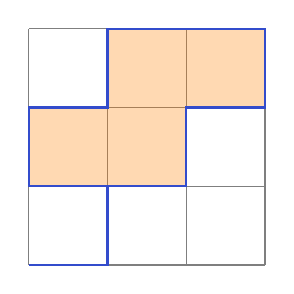
\begin{tikzpicture}
    \draw [step=1, opacity=0.5] (0, 0) grid (3, 3);

    \draw [thick, mblue, fill=morange, fill opacity=0.3] (0, 0) -- (1, 0) -- (1, 1) -- (2, 1) -- (2, 2) -- (3, 2) -- (3, 3) -- (1, 3) -- (1, 2) -- (0, 2) -- (0, 1) -- (1, 1) -- (1, 0) -- (0, 0);
  \end{tikzpicture}
\end{center}
We saw, at least heuristically, the algebraic area of $w$ is just the geometric area of this figure. Of course, sometimes it is slightly more complicated. For example, if we have the word $w = [a, b]^2$, then we have to use the cell $[a, b]$ twice.
%
%\begin{eg}
%  Take $\Gamma = \Z^2 \cong \bra a, b \mid [a, b]\ket$. Drawing this out:
%  \begin{center}
%    \begin{tikzpicture}
%      \draw [step=1, opacity=0.5] (-2, -2) grid (4, 4);
%
%      \draw [->] (-2, 0) -- (4, 0);
%      \draw [->] (0, -2) -- (0, 4);
%
%      \draw [->-=0.5] (0, 0) -- (1, 0) node [pos=0.5, below] {$a$};
%      \draw [->-=0.5] (0, 0) -- (0, 1) node [pos=0.5, left] {$b$};
%    \end{tikzpicture}
%  \end{center}
%  A null-homotopic word $w$ is then a loop in this diagram:
%  \begin{center}
%    \begin{tikzpicture}
%      \draw [step=1, opacity=0.5] (-2, -2) grid (4, 4);
%
%      \draw [->] (-2, 0) -- (4, 0);
%      \draw [->] (0, -2) -- (0, 4);
%
%      \draw [->-=0.5] (0, 0) -- (1, 0) node [pos=0.5, below] {$a$};
%      \draw [->-=0.5] (0, 0) -- (0, 1) node [pos=0.5, left] {$b$};
%
%      \draw [thick, mblue] (0, 0) -- (1, 0) -- (1, 1) -- (2, 1) -- (2, 2) -- (3, 2) -- (3, 3) -- (1, 3) -- (1, 2) -- (0, 2) -- (0, 1) -- (1, 1) -- (1, 0) -- (0, 0);
%    \end{tikzpicture}
%  \end{center}
%  The area of $W$ is just the area we have to fill in, $\Area(w) \leq 4$.
%
%  So to compute the Dehn function, we need to know what is the largest region we can fill with a path of length $n$. But this is just some classical geometry. We know that the most optimal way of doing so is by using a circle. In this case a loop of length $\ell$ can be filled in with area $\preccurlyeq \ell^2$. This is the \term{isoperimetric inequality}.
%
%  Of course, we cannot really draw a circle in $\Z^2$, but if we view the Dehn function only up to $\approx$, then it doesn't really matter, and $\delta_{\Z^2} \approx n^2$.
%
%\end{eg}
%
%\begin{eg}
%  In the same $\Z^2 \cong \bra a, b \mid [a, b] \ket$, and $w = [a, b]^2$, then $w$ is not embedded in $\R^2$, and we have to use the cell of $\R^2$ twice.
%\end{eg}
%
%How can we make this more rigorous? The key concept here is that of a \emph{singular disk diagram}.

\begin{defi}[Singular disc diagram]\index{singular disc diagram}\index{disc diagram}
  A \emph{(singular) disc diagram} is a compact, contractible subcomplex of $\R^2$, e.g.
  \begin{center}
    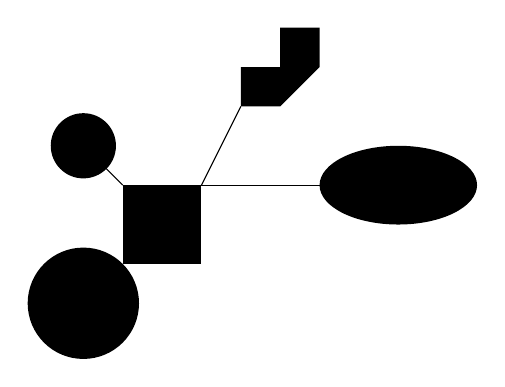
\begin{tikzpicture}
      \fill (0, 0) rectangle (1, 1);
      \draw (1, 1) -- (2.5, 1);
      \fill (3.5, 1) ellipse (1 and 0.5);
      \draw (1, 1) -- (1.5, 2);
      \fill (1.5, 2) -- (2, 2) -- (2.5, 2.5) -- (2.5, 3) -- (2, 3) -- (2, 2.5) -- (1.5, 2.5) -- (1.5, 2);

      \draw (0, 1) -- (-0.5, 1.5);
      \fill (-0.5, 1.5) circle [radius=0.414];

      \fill (-0.5, -0.5) circle [radius=0.707];
    \end{tikzpicture}
  \end{center}
  We usually endow the disc diagram $D$ with a base point $p$, and define
  \[
    \Area_g(D) = \text{number of $2$-cells of $D$}
  \]
  and
  \[
    \Diam_p(D) = \text{length of the longest embedded path in $D^{(1)}$, starting at $p$}.
  \]
  If we orient $\R^2$, then $D$ has a well-defined boundary cycle. A disc diagram is \emph{labelled} if each (oriented) edge is labelled by an element $s \in S^{\pm}$. The set of \term{face labels} is the set of boundary cycles of the $2$-cells.

  If all the face labels are elements of $R^{\pm}$, then we say $D$ is a \emph{diagram} over $\bra S \mid R\ket$.
\end{defi}


\begin{defi}[van Kampen diagram]\index{van Kampen diagram}
  If $w \in \bra \bra R \ket \ket$, and $w$ is the boundary cycle of a singular disc diagram $D$ over the presentation $\bra S \mid R\ket$, we say that $D$ is a \emph{van Kampen diagram} for $w$.
\end{defi}
\begin{eg}
  The diagram
  \begin{center}
    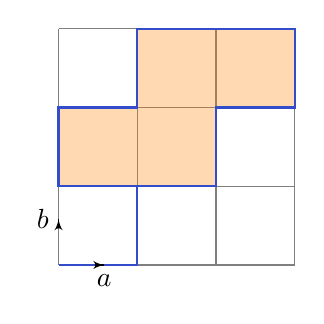
\begin{tikzpicture}
      \draw [step=1, opacity=0.5] (0, 0) grid (3, 3);

      \draw [thick, mblue, fill=morange, fill opacity=0.3] (0, 0) -- (1, 0) -- (1, 1) -- (2, 1) -- (2, 2) -- (3, 2) -- (3, 3) -- (1, 3) -- (1, 2) -- (0, 2) -- (0, 1) -- (1, 1) -- (1, 0) -- (0, 0);

      \draw [-latex'] (0.58, 0) -- +(0.001, 0) node [below] {$a$};
      \draw [-latex'] (0, 0.58) -- +(0, 0.001) node [left] {$b$};
    \end{tikzpicture}
  \end{center}
  is a van Kampen diagram for $abababa^{-2}b^{-1} a^{-1}b^{-1}ab^{-1}a^{-1}$.
\end{eg}

Note that in this case, the map $S^1 \to X_{\mathcal{P}}$ that represents $w$ factors through a map $D \to X_\mathcal{P}$.

\begin{lemma}[van Kampen's lemma]\index{van Kampen's lemma}
  Let $\mathcal{P} = \bra S \mid R\ket$ be a presentation and $w \in S^*$. Then the following are equivalent:
  \begin{enumerate}
    \item $w = 1$ in $\Gamma$ presented by $\mathcal{P}$ (i.e.\ $w$ is null-homotopic)
    \item There is a van Kampen diagram for $w$ given $\mathcal{P}$.
  \end{enumerate}
  If so, then
  \[
    \Area_a(w) = \min \{\Area_g(D): D\text{ is a van Kampen diagram for $w$ over $\mathcal{P}$}\}.
  \]
\end{lemma}

\begin{proof}
%  First observe that we may assume that $w$ is reduced, since if we have a non-reduced word, then in the van Kampen diagram, there must be a path segment that immediately backtracks itself, and we can just cancel them. This does not affect the area of the diagram.
  In one direction, given
  \[
    w = \prod_{i = 1}^n g_i r_i^{\pm} g_i^{-1} \in F(S)
  \]
  such that $w = 1 \in \Gamma$, we start by writing down a ``lollipop diagram''
  \begin{center}
    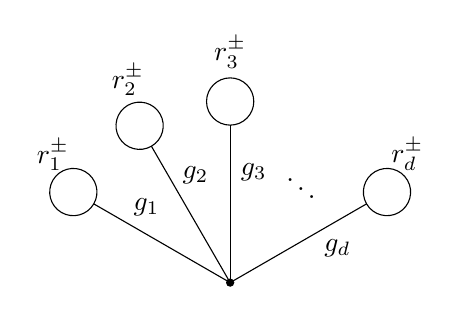
\begin{tikzpicture}
      \node [circ] {};

      \foreach \x/\lab in {-60/d,0/3,30/2,60/1} {
        \begin{scope}[rotate=\x]
          \draw (0, 0) -- (0, 2);

          \node at (0.3, 1.4) {$g_\lab$};
          \draw (0, 2.3) circle [radius=0.3];
          \node [above] at (0, 2.6) {$r_\lab^{\pm}$};
        \end{scope}
      }

      \node at (0.9, 1.3) {$\ddots$};
    \end{tikzpicture}
  \end{center}
  This defines a diagram for the word $\prod_{i = 1}^n g_i r_i^{\pm} g_i^{-1}$ which is equal in $F(S)$ to $w$, but is not exactly $w$. However, note that performing elementary reductions (or their inverses) correspond to operations on the van Kampen diagram that does not increase the area. We will be careful and not say that the area doesn't change, since we may have to collapse paths that look like
    \begin{center}
    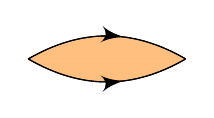
\begin{tikzpicture}
      \draw (0, 0) edge [bend left, fill=morange, fill opacity=0.5] (2, 0);
      \draw (2, 0) edge [bend left, fill=morange, fill opacity=0.5] (0, 0);
      \draw (0, 0) edge [bend left, ->-=0.6] (2, 0);
      \draw (0, 0) edge [bend right, ->-=0.6] (2, 0);
    \end{tikzpicture}
  \end{center}
%
%  $w' \underset{F(S)}{=} w$. Note that $\Area(D') = d$. We next need to define moves on diagrams to transform $w'$ to $w$. These are
%  \begin{itemize}
%    \item Pruning: We replace
%      \begin{center}
%        \begin{tikzpicture}
%          \fill [gray] circle [radius=0.5];
%          \draw [->-=0.5] (0.5, 0) -- (1.5, 0) node [pos=0.5, above] {$s$};
%        \end{tikzpicture}
%      \end{center}
%      with
%      \begin{center}
%        \begin{tikzpicture}
%          \fill [gray] circle [radius=0.5];
%        \end{tikzpicture}
%      \end{center}
%    \item Folding: If we see
%      \begin{center}
%        \begin{tikzpicture}
%          \draw [->-=0.5] (0, 0) -- (1, 0.5) node [pos=0.5, above] {$s$};
%          \draw [->-=0.5] (0,0 0) -- (1, -0.5) node [pos=0.5, below] {$s$};
%
%          \draw [red] (1, 0.5) -- (2, 2);
%          \draw [blue] (1, -0.5) -- (2, -2);
%        \end{tikzpicture}
%      \end{center}
%      We replace it with
%      \begin{center}
%        \begin{tikzpicture}
%          \draw [->-=0.5] (0, 0) -- (1, 0) node [pos=0.5, above] {$s$};
%
%          \draw [red] (1, 0) -- (2, 2);
%          \draw [blue] (1, 0) -- (2, -2);
%        \end{tikzpicture}
%      \end{center}
%  \end{itemize}
%  Note that if we see something that looks like
%  \begin{center}
%    \begin{tikzpicture}
%      \fill [gray] (0, 0) edge [bend left] (2, 0) edge [bend left] (0, 0); % this is going to be wrong
%      \draw (0, 0) edge [bend left, ->-=0.5] (2, 0) node [pos=0.5, above] {$s$};
%      \draw (0, 0) edge [bend right, ->-=0.5] (2, 0) node [pos=0.5, above] {$s$};
%    \end{tikzpicture}
%  \end{center}
%  folding replaces it with simply
%  \begin{center}
%    \begin{tikzpicture}
%      \draw [->-=0.5] (0, 0) -- (2, 0) node [pos=0.5, above] {$s$};
%    \end{tikzpicture}
%  \end{center}
%  Note that in this step, we lose area.
%
%  We see that we can perform one of moves whenever the boundary of our diagram forms a non-reduced word, and each of these moves corresponds to reducing the words. Therefore the procedure terminates and in the end, we obtain a diagram $D$ with boundary cycle $w$ and
%  \[
%    \Area(D) \leq \Area(D').
%  \]
%  % in each step, either area decreases or length decreases

  In the other direction, given a diagram $D$ for $w$, we need to produce an expression
  \[
    w = \prod_{i = 1}^d g_i r_i^{\pm} g_i^{-1}
  \]
  such that $d \leq \Area(D)$.

  We let $e$ be the first $2$-cell that the boundary curve arrives at, reading anticlockwise around $\partial D$. Let $g$ be the path from $p$ to $e$, and let $r$ be the relator read anti-clockwise around $e$. Let
  \[
    D' = D - e,
  \]
  and let $w' = \partial D'$. Note that
  \[
    w = gr^{\pm 1} g^{-1} w'.
  \]
  Since $\Area(D') = \Area(D) - 1$, we see by induction that
  \[
    w = \prod_{i = 1}^d g_i r_i^{\pm 1} g_i^{-1}
  \]
  with $d = \Area(D)$.
\end{proof}

We observe that in our algorithm about, the $g_i$'s produced have length $\leq \Diam(D)$. So we see that
\begin{cor}
  If $w$ is null-homotopic, then we can write $w$ in the form
  \[
    w = \prod_{i = 1}^d g_i r_i^{\pm} g_i^{-1},
  \]
  where
  \[
    |g_i|_S \leq \Diam D
  \]
  with $D$ a minimal van Kampen diagram for $w$. We can further bound this by
  \[
    (\max |r_i|_S) \Area(D) + |w|_S \leq \text{constant} \cdot \delta_{\mathcal{P}}(|w|_S) + |w|_S.
  \]
\end{cor}
So in particular, if we know $\delta_{\mathcal{P}}(|w|_S)$, then we can bound the maximum length of $g_i$ needed.

It is now easy to prove that
\begin{prop}
  The word problem for a presentation $\mathcal{P}$ is solvable iff $\delta_{\mathcal{P}}$ is computable.
\end{prop}

\begin{proof}\leavevmode
  \begin{itemize}
    \item[$(\Leftarrow)$] By the corollary, the maximum length of a conjugator $g_i$ that we need to consider is computable. Therefore we know how long the partial algorithm needs to run for.
    \item[$(\Rightarrow)$] To compute $\delta_{\mathcal{P}}(n)$, we use the word problem solving ability to find all null-homotopic words in $F(S)$ of length $\leq n$. Then for each $d$, go out and look for expressions
      \[
        w = \prod_{i = 1}^d g_i r_i^{\pm 1} g_i^{-1}.
      \]
      A naive search would find the smallest area expression, and this gives us the Dehn function.
  \end{itemize}
\end{proof}

It is a hard theorem that
\begin{thm}[Novikov--Boone theorem]\index{Novikov--Boone theorem}
  There exists a finitely-presented group with an unsolvable word problem.
\end{thm}

\begin{cor}
  $\delta_{\mathcal{P}}$ is sometimes non-computable.
\end{cor}

Let's look at some applications to geometry. In geometry, people wanted to classify manifolds. Classifying (orientable) $2$-dimensional manifolds is easy. They are completely labeled by the genus. This classification can in fact be performed by a computer. If we manage to triangulate our manifold, then we can feed the information of the triangulation into a computer, and then the computer can compute the Euler characteristic.

Is it possible to do this in higher dimensions? It turns out the word problem gives a severe hindrance to doing so.
\begin{thm}
  Let $n \geq 4$ and $\Gamma = \bra S \mid R\ket$ be a finitely-presented group. Then we can construct a closed, smooth, orientable manifold $M^n$ such that $\pi_1 M \cong \Gamma$.
\end{thm}
This is a nice, little surgery argument.

\begin{proof}
  Let $S = \{a_1, \ldots, a_m\}$ and $R = \{r_1, \ldots, r_n\}$. We start with
  \[
    M_0 = \#_{i = 0}^m (S^1 \times S^{n - 1}).
  \]
  Note that when we perform this construction, as $n \geq 3$, we have
  \[
    \pi_1M_0 \cong F_m
  \]
  by Seifert van-Kampen theorem. We now construct $M_k$ from $M_{k - 1}$ such that
  \[
    \pi_1 M_k \cong \bra a_1, \ldots, a_m \mid r_1, \ldots, r_k\ket.
  \]
  We realize $r_k$ as a loop in $M_{k - 1}$. Because $n \geq 3$, we may assume (after a small homotopy) that this is represented by a smooth embedded map $r_k: S^1 \to M_{k - 1}$.

  We take $N_k$ to be a smooth tubular neighbourhood of $r_k$. Then $N_k \cong S^1 \times D^{n - 1} \subseteq M_{k - 1}$. Note that $\partial N_k \cong S^1 \times S^{n - 2}$.

  Let $U_k = D^2 \times S^{n - 2}$. Notice that $\partial U_k \cong \partial N_k$. Since $n \geq 4$, we know $U_k$ is simply connected. So we let
  \[
    M'_{k - 1} = M_k \setminus \mathring{N}_k,
  \]
  a manifold with boundary $S^1 \times S^{n - 2}$. Choose an orientation-reversing diffeomorphism $\varphi_k: \partial U_k \to \partial M_{k - 1}'$. Let
  \[
    M_k = M_{k - 1}' \cup_{\varphi_k} U_k.
  \]
  Then by applying Seifert van Kampen repeatedly, we see that
  \[
    \pi_1 M_k = \pi_1 M_{k - 1} / \bra \bra r_k \ket \ket,
  \]
  as desired.
\end{proof}
Thus, if we have an algorithm that can distinguish between the fundamental groups of manifolds, then that would solve (some variant of) the word problem for us, which is impossible.

Finally, we provide some (even more) geometric interpretation of the Dehn function.

\begin{defi}[Filling disc]\index{filling disc}
  Let $(M, g)$ be a closed Riemannian manifold. Let $\gamma: S^1 \to M$ be a smooth null-homotopic loop. A filling disk for $\gamma$ in $M$ is a smooth map $f: D^2 \to M$ such that the diagram
  \[
    \begin{tikzcd}
      S^1 \ar[d, hook] \ar[rd, "\gamma"] \\
      D^2 \ar[r, "f"] & M
    \end{tikzcd}
  \]
\end{defi}

Since there is a metric $g$ on $M$, we can pull it back to a (possibly degenerate) metric $f^* g$ on $D^2$, and hence measure quantities like the length $\ell(\gamma)$ of $\gamma$ and the area $\Area(f)$ of $D^2$.

A classic result is
\begin{thm}[Douglas, Rad\'u, Murray] % check
  If $\gamma$ is embedded, then there is a least-area filling disc.
\end{thm}
So we can define
\begin{defi}[$\FArea$]\index{$\FArea$}
  \[
    \FArea(\gamma) = \inf \{\Area(f) \mid f: D^2 \to M\text{ is a filling disc for }\gamma\}.
  \]
\end{defi}

\begin{defi}[Isoperimetric function]\index{isoperimetric function}
  The isoperimetric function of $(M, g)$ is
  \begin{multline*}
    FiU^M: [0, \infty) \to [0, \infty)\\
    \ell \mapsto \sup\{\FArea(\gamma): \gamma: S^1 \to M\text{ is a smooth null-homotopic loop, }\ell(\gamma) \leq \ell\}
  \end{multline*}
\end{defi}

\begin{thm}[Filling theorem]
  let $M$ be a closed Riemannian manifold. Then $FiU^M \simeq \delta_{\pi_1 M}$.
\end{thm}

By our previous construction, we know this applies to every finitely-presented group.
%This theorem applies to every finitely-presented group, because
%\begin{thm}
%  If $n \geq 4$ and $\Gamma = \bra S \mid R\ket$ is a finitely-presented group, then there exists a closed, smooth, orientable manifold $M^n$ such that $\pi_1 M \cong \Gamma$.
%\end{thm}
%This is a nice, little surgery argument.
%
%\begin{proof}
%  Let $S = \{a_1, \ldots, a_m\}$ and $R = \{r_1, \ldots, r_n\}$. We start with
%  \[
%    M_0 = \#_{i = 0}^m (S^1 \times S^{n - 1}.
%  \]
%  Note that when we perform this construction, as $n \geq 3$, we have
%  \[
%    \pi_1M_0 \cong F_m
%  \]
%  by Seifert van-Kampen theorem. We now construct $M_k$ from $M_{k - 1}$ such that
%  \[
%    \pi_1 M_k \cong \bra a_1, \ldots, a_m \mid r_1, \ldots, r_k\ket.
%  \]
%  We realize $R_k$ as a loop in $M_{k - 1}$, which we may assume is null-homotopic. Because $n \geq 3$, we may assume (after a small homotopy) that this is represented by a smooth embedded map $r_k: S^1 \to M_{k - 1}$.
%
%  We take $N_k$ to be a smooth tubular neighbourhood of $r_k$. Then $N_k \cong S^1 \times D^{n - 1} \subseteq M_{k - 1}$. Note that $\partial N_k \cong S^1 \times S^{n - 2}$.
%
%  Let $U_k = D^2 \times S^{n - 2}$. Notice that $\partial U_k \cong \partial N_k$. Since $n \geq 4$, we know $U_k$ is simply connected. So we let
%  \[
%    M'_{k - 1} = M_k \setminus \mathring{N}_k,
%  \]
%  a manifold with boundary $S^1 \times S^{n - 2}$. Choose an orientation-reversing diffeomorphism $\varphi_k: \partial U_k \to \partial M_{k - 1}'$. Let
%  \[
%    M_k = M_{k - 1}' \cup_{\varphi_k} U_k.
%  \]
%  Then by applying Seifert van Kampen repeatedly, we see that
%  \[
%    \pi_1 M_k = \pi_1 M_{k - 1} / \bra \bra r_k \ket \ket,
%  \]
%  as desired.
%\end{proof}
%
%The point is that whenever we come up with a bad group, we can construct a bad manifold with similar bad behaviour. So manifolds are at least as difficult to understand as groups. In particular, there is no algorithm that can distinguish any two smooth manifolds, since that would allow us to figure out if two group presentations define the same group, which we know is impossible.

\section{New groups from old: A crash course in Bass--Serre theory}
The idea is that we want to be able to do things similar to how we built new manifolds by gluing together old manifolds.

\subsection{Graphs of spaces}
Disclaimer: All spaces are cell complexes.

We want to build new spaces by gluing well-understood spaces together via homotopy pushouts.

\begin{defi}[Homotopy pushout]\index{homotopy pushout}
  Let $X, Y, Z$ be spaces, and $\partial^-: Z \to X$ and $\partial^+: Z \to Y$ be maps. We define\index{$X \underset{Z}{\coprod} Z$}
  \[
    X \underset{Z}{\coprod} Y = (X \coprod Y \coprod Z \times [-1, 1])/\sim,
  \]
  where we identify $\partial^{\pm}(z)\sim (z, \pm 1)$ for all $z \in Z$.
\end{defi}
% insert picture
\begin{center}
  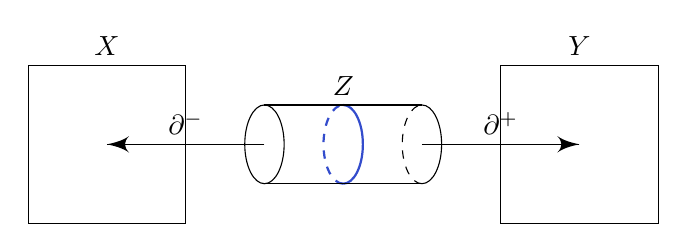
\begin{tikzpicture}
    \draw (0, 0) rectangle (2, 2);
    \draw (6, 0) rectangle (8, 2);

    \draw (3, 1) ellipse (0.25 and 0.5);

    \draw [thick, mblue] (4, 0.5) arc(-90:90:0.25 and 0.5);
    \draw [dashed, thick, mblue] (4, 0.5) arc(270:90:0.25 and 0.5);

    \draw (5, 0.5) arc(-90:90:0.25 and 0.5);
    \draw [dashed] (5, 0.5) arc(270:90:0.25 and 0.5);

    \draw (3, 0.5) -- (5, 0.5);
    \draw (3, 1.5) -- (5, 1.5);

    \draw [->] (3, 1) -- (1, 1) node [pos=0.5, above] {$\partial^-$};
    \draw [->] (5, 1) -- (7, 1) node [pos=0.5, above] {$\partial^+$};

    \node [above] at (1, 2) {$X$};
    \node [above] at (7, 2) {$Y$};
    \node [above] at (4, 1.5) {$Z$};
  \end{tikzpicture}
\end{center}
By Seifert van-Kampen, we know $\pi_1(X\underset{Z}{\coprod} Y)$ is the pushout
\[
  \begin{tikzcd}
    \pi_1Z \ar[r, "\partial^+_*"] \ar[d, "\partial^-_*"] & X \ar[d]]\\
    \pi_1 Y \ar[r] & \pi_1(X \underset{Z}{\coprod} Y)
  \end{tikzcd}
\]
If $\pi_*^{\pm}$ are injective, then we have
\[
  \pi_1(X \underset{Z}{\coprod} Y) \cong \pi_1 X \underset{\pi_1 Z}{*} \pi_1Y.
\]
We want to generalize this.

\begin{defi}[Graph of spaces]\index{graph!of spaces}
  A \emph{graph of spaces} $\mathcal{X}$ consists of the following data
  \begin{itemize}
    \item A connected graph $\Xi$.
    \item For each vertex $v \in V(\Xi)$, a path-connected space $X_v$.
    \item For each edge $e \in E(\Xi)$, a path-connected space $X_e$.
    \item For each edge $e \in E(\Xi)$ attached to $v^{\pm} \in V(\Xi)$, we have $\pi_1$-injective maps $\partial^{\pm}_e : X_e \to X_{v^{\pm}}$.
  \end{itemize}
  The \term{realization} of $\mathcal{X}$ is
  \[
    |\mathcal{X}| = X = \coprod_{v \in V(\Xi)} X_v \amalg \coprod_{e \in E(\Xi)} (X_e \times [-1, ]1)/(\forall e \in E(\Xi), \forall x \in X_e, (x, \pm 1) \sim \partial_e^{\pm}(x)).
  \]
\end{defi}
These conditions are not too restrictive. If our vertex or edge space were not path-connected, then we can just treat each path component as a separate vertex/edge. If our maps are not $\pi_1$ injective, as long as we are careful enough, we can attach $2$-cells to kill the relevant loops.


\begin{eg}
  Let $X$ be an orientable surface and $Y$ be a multi-curve, i.e. a disjoint union of essentially simple closed curves on $X$. Take a tubular neighbourhood of each curve in $Y$, and let $N(Y)$ be the union of all these tubular neighbourhoods, which is a union of closed annuli. Let
  \[
    \coprod X_i = X - \mathring{N(Y)}
  \]
  be the decomposition of $X - \mathring{N(Y)}$ into connected components.

  % insert picture

  We can then take $\coprod X_e = Y$. Then $X$ is just the realization of this graph, when we pick the appropriate attaching maps.
\end{eg}

\begin{eg}
  In the case of
  \begin{center}
    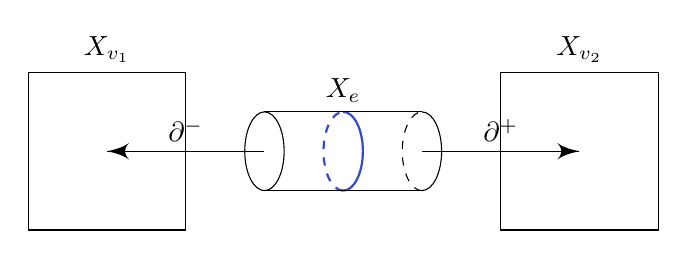
\begin{tikzpicture}
      \draw (0, 0) rectangle (2, 2);
      \draw (6, 0) rectangle (8, 2);

      \draw (3, 1) ellipse (0.25 and 0.5);

      \draw [thick, mblue] (4, 0.5) arc(-90:90:0.25 and 0.5);
      \draw [dashed, thick, mblue] (4, 0.5) arc(270:90:0.25 and 0.5);

      \draw (5, 0.5) arc(-90:90:0.25 and 0.5);
      \draw [dashed] (5, 0.5) arc(270:90:0.25 and 0.5);

      \draw (3, 0.5) -- (5, 0.5);
      \draw (3, 1.5) -- (5, 1.5);

      \draw [->] (3, 1) -- (1, 1) node [pos=0.5, above] {$\partial^-$};
      \draw [->] (5, 1) -- (7, 1) node [pos=0.5, above] {$\partial^+$};

      \node [above] at (1, 2) {$X_{v_1}$};
      \node [above] at (7, 2) {$X_{v_2}$};
      \node [above] at (4, 1.5) {$X_e$};
    \end{tikzpicture}
  \end{center}
  Recall that Seifert--van Kampen tells us
  \[
    \pi_1 X \cong \pi_1 X_{v_1} \underset{\pi_1 X_e}{*} \pi_1 X_{v_2}.
  \]
\end{eg}

\begin{eg}
  If we instead have

  % insert picture with single self-loop

  then if we think carefully, we find that we have
  \[
    \pi_1 X = \frac{\pi_1 X_v * \bra t\ket}{\bra \bra(\partial_e^+)_*(g) = t (\partial_e^-)_*(g) t^{-1} \forall g \in \pi_1 X_e\ket \ket}.
  \]
  Here $t$ represents a loop that starts at $X_v$, goes around $X_e$, and returns to the original point in $X_v$.

  This is known as an \term{HNN extension}. The way to think about this is as follows --- we have a group $\pi_1 X_v$, and we have two subgroups that are isomorphic to each other. Then the HNN extension is the ``free-est'' way to modify the group so that these two subgroups are conjugate.
\end{eg}

How about for a general graph of spaces? If $\Xi$ is a graph of spaces, then its fundamental group has the structure of a \emph{graph of groups} $\mathcal{G}$.

\begin{defi}[Graph of groups]\index{graph!of groups}
  A \emph{graph of groups} $\mathcal{G}$ consists of
  \begin{itemize}
    \item A graph $\Gamma$
    \item Groups $G_v$ for all $v \in V(\Gamma)$
    \item Groups $G_e$ for all $e \in E(\Gamma)$
    \item For each $e \mapsto v^{\pm}(e)$, injective group homomorphisms
      \[
        \partial_e^{\pm}: G_e \to G_{v^{\pm}(e)}.
      \]
  \end{itemize}
\end{defi}
In the case of a graph of spaces, it was easy to define a realization. One way to do so is that we have already see how to do so in the two above simple cases, and we can build the general case up inductively from the simple cases, but that is not so canonical. However, this has a whole lot of choices involved. Instead, we are just going to do is to associate to a graph of groups $\mathcal{G}$ a graph of spaces $\mathcal{X}$ which ``inverts'' the natural map from graphs of spaces to graphs of groups, given by taking $\pi_1$ of everything.

This can be done by taking Eilenberg--Maclane spaces.
\begin{defi}[Aspherical space]\index{aspherical space}
  A space $X$ is \emph{aspherical} if $\tilde{X}$ is contractible. By Whitehead's theorem and the lifting criterion, this is true iff $\pi_n(X) = 0$ for all $n \geq 2$.
\end{defi}

\begin{prop}
  For all groups $G$ there exists an aspherical space $BG = K(G, 1)$\index{$BG$}\index{$K(G, 1)$} such that $\pi_1(K(G, 1)) \cong G$. Moreover, for any two choices of $K(G, 1)$ and $K(H, 1)$, and for every homomorphism $f: G \to H$, there is a unique map (up to homotopy) $\bar{f}: K(G, 1) \to K(H, 1)$ that induces this homomorphism on $\pi_1$. In particular, $K(G, 1)$ is well-defined up to homotopy equivalence.

  Moreover, we can choose $K(G, 1)$ functorially, namely there are choices of $K(G, 1)$ for each $G$ and choices of $\bar{f}$ such that $\overline{f_1 \circ f_2} = \overline{f}_1 \circ \bar{f}_2$ and $\overline{\id_{G}} = \id_{K(G, 1)}$ for all $f, G, H$.
\end{prop}
When we talked about presentations, we saw that this is true if we don't have the word ``aspherical''. But the aspherical requirement makes the space unique.

These $K(G, 1)$ are known as \term{Eilenberg--MacLane spaces}
\begin{proof}
  See Hatcher (or Segal (or May)).
\end{proof}

Using Eilenberg--MacLane spaces, given any graph of groups $\mathcal{G}$, we can construct a graph of spaces $\Xi$ such that when we apply $\pi_1$ to all the spaces in $\mathcal{X}$, we recover $\mathcal{G}$.

We can now set
\[
  \pi_1 \mathcal{G} = \pi_1|\mathcal{X}|.
\]
For more details, read \emph{Trees} by Serre, or \emph{Topological methods in group theory} by Scott and Wall.

Note that if $\Gamma$ is finite, and all the $G_v$'s are finitely-generated, then $\pi_1\mathcal{G}$ is also finitely-generated, which one can see by looking into the construction of $K(G, 1)$. If $\Gamma$ is finite, all $G_v$'s are finitely-presented and all $G_e$'s are finitely-generated, then $\pi_1 \mathcal{G}$ is finitely-presented.

\subsection{The Bass--Serre tree}
Given a graph of groups $\mathcal{G}$, we want to analyze $\pi_ 1\mathcal{G} = \pi_1 X$, and we do this by the natural action of $G$ on $\tilde{X}$ by deck transformations.

Recall that to understand the free group, we looked at the universal cover of the rose with $r$ petals. Since the rose was a graph, the universal cover is also a graph, and because it is simply connected, it must be a tree, and this gives us a normal form theorem. The key result was that the covering space of a graph is a graph.

\begin{lemma}
  If $\mathcal{X}$ is a graph of spaces and $\hat{X} \to X$ is a covering map, then $\hat{X}$ naturally has the structure of a graph of spaces $\hat{\mathcal{X}}$, and $p$ respects that structure.
\end{lemma}
Note that the underlying graph of $\hat{\mathcal{X}}$ is not necessarily a covering space of the underlying graph of $\mathcal{X}$.

\begin{proof}[Proof sketch]
  Consider
  \[
    \bigcup_{v \in V(\Xi)} X_V \subseteq X.
  \]
  Let
  \[
    p^{-1}\left(\bigcup_{v \in V(\Xi)} X_V\right) = \coprod_{\hat{v} \in V(\hat{\Xi})} \hat{W}_{\hat{v}}.
  \]
  This defines the vertices of $\hat{\Xi}$, the underlying graph of $\hat{\mathcal{X}}$. The path components $\hat{X}_{\hat{v}}$ are going to be the vertex spaces of $\hat{\mathcal{X}}$. Note that for each $\hat{v}$, there exists a unique $v \in V(\Xi)$ such that $p: \hat{X}_{\hat{v}} \to X_v$ is a covering map.

  Likewise, the path components of
  \[
    p^{-1}\left(\bigcup_{e \in E(\Xi)} X_e \times \{0\}\right)
  \]
  form the edge spaces $\coprod_{e \in E(\Xi)} \hat{X}_{\hat{e}}$ of $\hat{\mathcal{X}}$, which again are covering spaces of the edge space of $X$.

  Now let's define the edge maps $\partial_{\hat{e}}^{\pm}$ for each $\hat{e} \in E(\hat{\Xi}) \mapsto e \in E(\Xi)$. To do so, we consider the diagram
  \[
    \begin{tikzcd}
      \hat{X}_{\hat{e}} \ar[r, hook, "\sim"] \ar[rr, bend left] \ar[d] & \hat{X}_{\hat{e}} \times [-1, 1] \ar[d] \ar[r, dashed] & \hat{X} \ar[d, "p"]\\
      X_e \ar[r, hook, "\sim"] & X_e \times [-1, 1] \ar[r] & X
    \end{tikzcd}
  \]
  By the lifting criterion, for the dashed map to exist, there is a necessary and sufficient condition on $(\hat{X}_{\hat{e}} \times [-1, 1] \to X_e \times [-1, 1] \to X)_*$. But since this condition is homotopy invariant, we can check it on the composition $(\hat{X}_{\hat{e}} \to X_e \to X)_*$ instead, and we know it must be satisfied because a lift exists in this case.

  The attaching maps $\partial^{\pm}_{\hat{e}}: \hat{X}_e \to \hat{X}$ are precisely the restriction to $\hat{X}_e \times \{\pm 1\} \to \hat{X}$.

  Finally, check using covering space theory that the maps $\hat{X}_{\hat{e}} \times [-1, 1] \to \hat{X}$ can injective on the interior of the cylinder, and verify that the appropriate maps are $\pi_1$-injective.
\end{proof}

Now let's apply this to the universal cover $\tilde{X} \to X$. We see that $\tilde{X}$ has a natural action of $G = \pi_1X$, which preserves the graph of spaces structure.

Note that for any graph of spaces $X$, there are maps
\begin{align*}
  \iota: \Xi &\to X\\
  \rho: X &\to \Xi
\end{align*}
such that $\rho \circ \iota \simeq \id_{\Xi}$. In particular, this implies $\rho_*$ is surjective (and of course $\rho$ itself is also surjective).

In the case of the universal cover $\tilde{X}$, we see that the underlying graph $\tilde{\Xi} = T$ is connected and simply connected, because $\pi_1 \tilde{\Xi} = \rho_*(\pi_1 \tilde{X}) = 1$. So it is a tree!

The action of $G$ on $\tilde{X}$ descends to an action of $G$ on $\tilde{\Xi}$. So whenever we have a graph of spaces, or a graph of groups $\mathcal{G}$, we have an action of the fundamental group on a tree. This tree is called the \term{Bass--Serre tree} of $\mathcal{G}$.

Just like the case of the free group, careful analysis of the Bass--Serre tree leads to theorems relating $\pi_1(\mathcal{G})$ to the vertex groups $G_v$ and edge groups $G_e$.

\begin{eg}
  Let
  \[
    G = F_2 = \bra a\ket * \bra b\ket = \Z * \Z.
  \]
  In this case, we take $X$ to be

  \begin{center}
    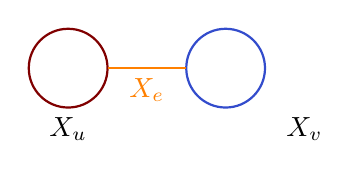
\begin{tikzpicture}
      \draw [mred, thick] circle [radius=0.5];
      \draw [mblue, thick] (2, 0) circle [radius=0.5];
      \draw [morange, thick] (0.5, 0) -- (1.5, 0) node [pos=0.5, below] {$X_e$};

      \node [below] at (0, -0.5) {$X_u$};
      \node [below] at (3, -0.5) {$X_v$};
    \end{tikzpicture}
  \end{center}
  Here we view this as a graph where the two vertex spaces are circles, and there is a single edge connecting them. The covering space $\tilde{X}$ then looks like
  \begin{center}
    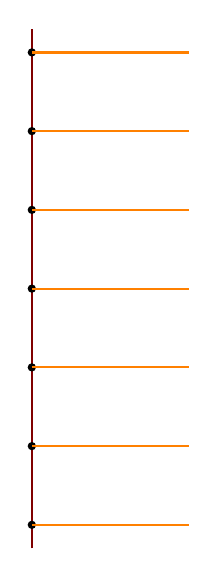
\begin{tikzpicture}
      \draw [mred, thick] (0, -3.3) -- (0, 3.3);
      \foreach \y in {-3,...,3} {
        \node [circ] at (0, \y) {};
        \draw [morange, thick] (0, \y) -- (2, \y);

%        \draw [mblue, thick] (2, \y-0.3) -- (2, \y + 0.3); % infinitely many yellow things pointing to the left.
      }
    \end{tikzpicture}
  \end{center}
  This is \emph{not} the Bass--Serre tree. The Bass--Serre tree looks like % insert picture

  Thus, this is an infinite-valent bipartite tree.
\end{eg}

The simply-connected of the Bass--Serre tree translates into a normal form for the elements of $G$.

This point of view gives two important results that relate elements of $G$ to the vertex groups $G_{v_i}$ and the edge maps $\partial_{e_j}^{\pm}: G_{e_j} \to G_{v_j^{\pm}}$.

\begin{lemma}[Britton's lemma]\index{Britton's lemma}
  For any vertex $\Xi$, the natural map $G_v \to G$ is injective.
\end{lemma}
Unsurprisingly, this really requires that the edge maps are injective. It is an exercise to find examples to show that this fails if the boundary maps are not injective.

\begin{proof}[Proof sketch]
  Observe that the universal cover $\tilde{X}$ can be produce by first building universal covers of the vertex space, which are then glued together in a way that doesn't kill the fundamental groups.
\end{proof}

The next theorem is a normal form theorem. Pick a base vertex $v \in V(\Xi)$. We can then represent elements of $G$ via loops in $\Xi = \Gamma$, the underlying graph based at $v$ and labelled by elements of vertex groups. These loops can be written formally as
\[
  \gamma = g_0 e_1^{\pm 1} g_1 e_2^{\pm 1} \cdots e_n^{\pm 1}g_n
\]
We say a \emph{pinch} is a sub-word of the form
\[
  e^{\pm 1} \partial_e^{\pm 1} (g) e^{\mp 1},
\]
which can be replaced by $\partial_e^{\mp 1}(g)$.

We say a loop is \emph{reduced} if it contains no pinches.

\begin{thm}[Normal form theorem]\index{normal form theorem}
  Every element can be represented by a reduced loop, and the only reduced loop representing the identity is the trivial loop.
\end{thm}
This is good enough, since if we can recognize is something is the identity, then we see if the product of one with the inverse of the other is the identity. An exact normal form for all words would be tricky.

\begin{proof}[Proof idea]
  It all boils down to the fact that the Bass--Serre tree is a tree. Connectedness gives the existence, and the simply-connectedness gives the ``uniqueness''.
\end{proof}

\section{Hyperbolic groups}
So far, we obtained a lot of information about groups by seeing how they act on trees. Philosophically, the reason for this is that trees are very ``negatively curved'' spaces. We shall see in this chapter than in general, whenever a group acts on a negatively curved space, we can learn a lot about the group.

\subsection{Definitions and examples}
We now want to define a negatively-curved space in great generality. Let $X$ be a geodesic metric space. Given $x, y \in X$, we will write $[x, y]$ for a choice of geodesic between $x$ and $y$.

\begin{defi}[Geodesic triangle]\index{geodesic triangle}\index{triangle!geodesic}
  A \emph{geodesic triangle} $\Delta$ is a choice of three points $x, y, z$ and geodesics $[x, y], [y, z], [z, x]$.
\end{defi}
Geodesic triangles look like this:
\begin{center}
  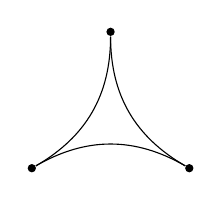
\begin{tikzpicture}
    \node [circ] (a) at (0, 0) {};
    \node [circ] (b) at (2, 0) {};
    \node [circ] (c) at (1, 1.732) {};

    \draw (a) edge [bend left] (b);
    \draw (b) edge [bend left] (c);
    \draw (c) edge [bend left] (a);
  \end{tikzpicture}
\end{center}
Note that in general, the geodesics may intersect.

\begin{defi}[$\delta$-slim triangle]\index{$\delta$-slim triangle}
  We say $\Delta$ is $\delta$-slim if every side of $\Delta$ is contained in the union of the $\delta$-neighbourhoods of the other two sides.
\end{defi}

\begin{defi}[Hyperbolic space]\index{hyperbolic space}\index{Gromov hyperbolic space}\index{$\delta$-hyperbolic space}
  A metric space is \emph{(Gromov) hyperbolic} if there exists $\delta \geq 0$ such that every geodesic triangle in $X$ is $\delta$-slim. In this case, we say it \emph{is $\delta$-hyperbolic}.
\end{defi}

\begin{eg}
  $\R^2$ is not Gromov hyperbolic.
\end{eg}

\begin{eg}
  If $X$ is a tree, then $X$ is $0$-hyperbolic! Indeed, each triangle looks like
  \begin{center}
    \begin{tikzpicture}
      \node [circ] (a) at (0, 0) {};
      \node [circ] (b) at (2, 0) {};
      \node [circ] (c) at (1, 1.732) {};

      \draw (a) -- (1, 0.866);
      \draw (b) -- (1, 0.866);
      \draw (c) -- (1, 0.866);
    \end{tikzpicture}
  \end{center}
  We call this a \term{tripod}.
\end{eg}
Unfortunately, none of these examples really justify why we call these things hyperbolic. Let's look at the actual motivating example.

\begin{eg}
  Let $X = \H^2$, the \term{hyperbolic plane}. Let $\Delta \subseteq \H^2$ be a triangle. Then $\Delta$ is $\delta$-slim, where the maximum radius of an inscribed semi-circle $D$ in $\Delta$ with the center on one of the edges.

  But we know that the radius of $D$ is bounded by some increasing function of the area of $D$, and the area of $D$ is bounded above by the area of $\Delta$. On the other hand, by hyperbolic geometry, we know the area of \emph{any} triangle is bounded by $\pi$.

  So $\H^2$ is $\delta$-hyperbolic for some $\delta$.
\end{eg}
For the arguments we are going to do, we don't really care about what $\delta$ is.

\begin{eg}
  Let $X$ be any bounded metric space, e.g.\ $S^2$. Then $X$ is Gromov hyperbolic, since we can just take $\delta$ to be the diameter of the metric space.
\end{eg}
This is rather silly, but it makes sense if we take the ``coarse point of view'', and we have to ignore bounded things.

What we would like to do is to say is that a group $\Gamma$ if for every finite generating set $S$, the Cayley graph $\Cay_S(\Gamma)$ equipped with the word metric is $\delta$-hyperbolic for some $\delta$.

However, this is not very helpful, since we have to check it for all finite generating sets. So we want to say that being hyperbolic is quasi-isometry invariant, in some sense.

This is slightly difficult, because we lose control of how the geodesic behaves if we only look at things up to isometry. To do so, we have to talk about quasi-geodesics.

\subsection{Quasi-geodesics and hyperbolicity}
\begin{defi}[quasi-geodesic]\index{quasi-geodesic}
  A $(\lambda, \varepsilon)$-quasi-geodesic for $\lambda \geq 1, \varepsilon \geq 0$ is a $(\lambda, \varepsilon)$-quasi-isometric embedding $I \to X$, where $I \subseteq \R$ is a closed interval.
\end{defi}
Note that our definition allows for $I$ to be unbounded, i.e.\ $I$ may be of the forms $[a, b]$, $[0, \infty)$ or $\R$ respectively. We call these \emph{quasi-geodesic intervals}\index{quasi-geodesic interval}, \emph{quasi-geodesic rays}\index{quasi-geodesic ray} and \emph{quasi-geodesic lines}\index{quasi-geodesic line} respectively.

\begin{eg}
  The map $[0, \infty) \to \R^2$ given in polar coordinates by
  \[
    t \mapsto (t, \log(1 + t))
  \]
  is a quasigeodesic ray.
\end{eg}
This should be alarming. The quasi-geodesics in the Euclidean plane can look unlike any genuine geodesic.

\begin{thm}[Morse lemma]\index{Morse lemma}
  For all $\delta \geq 0, \lambda \geq 1$ there is $R(\delta, \lambda, \varepsilon)$ such that the following holds:

  If $X$ is a $\delta$-hyperbolic metric space, and $c: [a, b] \to X$ is a $(\lambda, \varepsilon)$-quasigeodesic from $p$ to $q$, and $[p, q]$ is a choice of geodesic from $p$ to $q$, then
  \[
    d_{Haus}([p, q], \im(c)) \leq R(\delta, \lambda, \varepsilon),
  \]
  where
  \[
    d_{Haus}(A, B) = \inf\{\varepsilon > 0 \mid A \subseteq N_\varepsilon(B) \text{ and }B \subseteq N_\varepsilon(A)\}
  \]
  is the \term{Hausdorff distance}\index{$d_{Haus}$}.
\end{thm}
This has nothing to do with the Morse lemma in differential topology.

\begin{cor}
  There is an $M(\delta, \lambda, \varepsilon)$ such that a geodesic metric space $X$ is $\delta$-hyperbolic iff any $(\lambda, \varepsilon)$-quasigeodesic triangle is $M$-slim.
\end{cor}

\begin{cor}
  Suppose $X, X'$ are geodesic metric spaces, and $f: X \to X''$ is a quasi-isometric embedding. If $X'$ is hyperbolic, then so is $X$.

  In particular, hyperbolicity is a quasi-isometrically invariant property, when restricted to geodesic metric spaces.
\end{cor}

Thus, we can make the following definition:
\begin{defi}[Hyperbolic group]\index{hyperbolic group}
  A group $\Gamma$ is \emph{hyperbolic} if it acts properly discontinuously and cocompactly by isometries on a proper, geodesic hyperbolic metric space. Equivalently, if it is finitely-generated and with a hyperbolic Cayley graph.
\end{defi}

Let's prove the Morse lemma. To do so, we need the following definition:
\begin{defi}[Length of path]\index{length of path}
  Let $c: [a, b] \to X$ be a continuous path. Let $a = t_0 < t_1 < \cdots < t_n = b$ be a \term{dissection} $\mathcal{D}$ of $[a, b]$. Define
  \[
    \ell (c) = \sup_{\mathcal{D}} \sum_{i = 1}^n d(c(t_{i - 1}), c(t_i)).
  \]
\end{defi}
In general, this number is extremely hard to compute, and may even be finite.

\begin{defi}[Rectifiable path]\index{rectifiable path}
  We say a path $c$ is \emph{rectifiable} if $\ell(c) < \infty$.
\end{defi}

\begin{eg}
  Piecewise geodesic paths are rectifiable.
\end{eg}

\begin{lemma}
  Let $X$ be a geodesic space. For any $(\lambda, \varepsilon)$-quasigeodesic $c: [a, b] \to X$, there exists a continuous, rectifiable $(\lambda, \varepsilon')$-quasigeodesic $c'[a, b] \to X$ with $\varepsilon' = 2(\lambda + \varepsilon)$ such that
  \begin{enumerate}
    \item $c'(a) = c(a)$, $c'(b) = c(b)$.
    \item For all $a \leq t < t' \leq b$, we have
      \[
        \ell(c'|_{[t, t']}) \leq k_1 d(c'(t), c'(t')) + k_2
      \]
      where $k_1 = \lambda (\lambda + \varepsilon)$ and $k_2 = (\lambda \varepsilon' + 3)(\lambda + 3)$.
    \item $d_{Haus}(\im c, \im c') \leq \lambda + \varepsilon$.
  \end{enumerate}
\end{lemma}

\begin{proof}[Proof sketch]
  Let $\Sigma = \{a, b\} \cup ((a, b) \cap \Z)$. For $t \in \Sigma$, we let $c'(t) = c(t)$, and define $c'$ to be geodesic between the points of $\Sigma$. Then claims (i) and (iii) are clear, and to prove quasigeodesicity and (ii), let $\sigma: [a, b] \to \Sigma$ be a choice of closest point in $\Sigma$, and then estimate $d(c'(t), c'(t'))$ in terms of $d(c(\sigma(t)), c(\sigma(t')))$.
\end{proof}

\begin{lemma}
  let $X$ be $\delta$-hyperbolic, and $c: [a, b] \to X$ a continuous, rectifiable path in $X$ joining $p$ to $q$. For $[p, q]$ a geodesic, for any $x \in [p, q]$, we have
  \[
    d(x, \im c) \leq \delta |\log_2\ell(c)| + 1.
  \]
\end{lemma}

\begin{proof}
  We may assume $c: [0, 1] \to X$ is parametrized proportional to arc length. Suppose
  \[
    \frac{\ell(c)}{2^N} < 1 \leq \frac{\ell(c)}{2^{N - 1}}.
  \]
  Let $x_0 = x$. Pick a geodesic triangle between $p, q, c(\frac{1}{2})$. By $\delta$-hyperbolicity, there exists a point $x_1$ lying on the other two edges such that $d(x_0, x_1) \leq \delta$. We wlog assume $x_1 \in [p, c(\frac{1}{2})]$. We can repeat the argument with $c|_{[0, \frac{1}{2}]}$.

  \begin{center}
    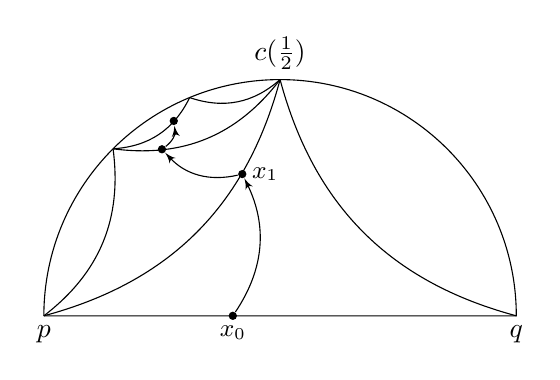
\begin{tikzpicture}[scale=1.5]
      \draw (-2, 0) -- (2, 0) arc(0:180:2);
      \node [below] at (-2, 0) {$p$};
      \node [below] at (2, 0) {$q$};
      \node [above] at (0, 2) {$c(\frac{1}{2})$};

      \draw (-2, 0) edge [bend right] (0, 2);
      \draw (0, 2) edge [bend right] (2, 0);

      \draw (-2, 0) edge [bend right] (-1.414, 1.414);
      \draw (-1.414, 1.414) edge [bend right] (0, 2);

      \draw (-1.414, 1.414) edge [bend right] (-0.7654, 1.8476);
      \draw (-0.7654, 1.8476) edge [bend right] (0, 2);

      \node [circ] (a) at (-0.4, 0) {};
      \node [below] at (-0.4, 0) {\small$x_0$};

      \node [circ] (b) at (-0.32, 1.2) {};
      \node [right] at (b) {\small$x_1$};

      \node [circ] (c) at (-1, 1.41) {};

      \node [circ] (d) at (-0.9, 1.65) {};

      \draw (a) edge [bend right, -latex'] (b);
      \draw (b) edge [bend left, -latex'] (c);
      \draw (c) edge [bend right, -latex'] (d);
      % insert points
    \end{tikzpicture}
  \end{center}

  Formally, we proceed by induction on $N$. If $N = 0$ so that $\ell(c) < 1$, then we are done by taking desired point on $\im c$ to be $p$ (or $q$). Otherwise, there is some $x_1 \in [p, c(\frac{1}{2})]$ such that $d(x_0, x_1) \leq \delta$. Then
  \[
    \frac{\ell(c|_{[0, \frac{1}{2}]})}{2^{N - 1}} < 1 \leq \frac{\ell(c|_{[0, \frac{1}2}])}{2^{N - 2}}.
  \]
  So by the induction hypothesis,
  \begin{align*}
    d(x_1, \im c) &\leq \delta |\log_2 \ell(c|_{[0, \frac{1}{2}]}| + 1\\
    &= \delta \abs{ \frac{1}{2}\log_2 \ell(c)} + 1\\
    &= \delta (\abs{\log_2 \ell(c)} - 1) + 1.
  \end{align*}
  Note that we used the fact that $\ell(c) > 1$, so that $\log_2 \ell(c) > 0$.

  Then we are done since
  \[
    d(x, \im c) \leq d(x, x_1) + d(x_1, \im c).
  \]
\end{proof}

\begin{proof}[Proof of Morse lemma]
  By the first lemma, we may assume that $c$ is continuous and rectifiable, and satisfies the properties as in the lemma.

  First, we show that $[p, q]$ is contained in a bounded neighbourhood of $\im c$. Let
  \[
    D = \sup\{d(x, \im c) \mid x \in [p, q]\}.
  \]
  Since $[p, q]$ and $\im c$ are compact, we can let $x_0$ be a point where the supremum is obtained.

  Let $p, q$ be the end points of $c$, and $[p, q]$ a geodesic. First we show that $[p, q]$ is contained in a bounded neighbourhood of $\im c$. Let
  \[
    D = \sup_{x \in [p, q]} d(x, \im c).
  \]
  By compactness of the interval, let $x_0 \in [p, q]$ where the supremum is attained. Then by assumption, $\im c$ lies outside $\mathring{B}(x_0, D)$. Choose $y, z \in [p, q]$ be such that $d(x_0, y) = d(x_0, z) = 2D$ and $y, x_0, z$ appear on the geodesic in this order (take $y = p$, or $z = q$ if that is not possible).

  Let $y' = c(s) \in \im c$ be such that $d(y', y) \leq D$, and similarly let $z' = c(t) \in \im c$ be such that $d(z, z') \leq D$.
  \begin{center}
    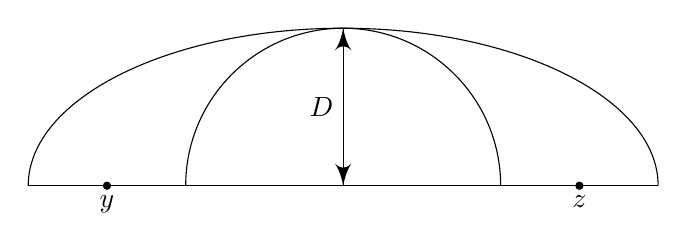
\begin{tikzpicture}
      \draw (-4, 0) arc(180:0:4 and 2);
      \draw (-4, 0) -- (4, 0);
      \draw (-2, 0) arc (180:0:2);

      \draw [<->] (0, 0) -- (0, 2) node [pos=0.5, left] {$D$};

      \node [circ] at (-3, 0) {};
      \node [below] at (-3, 0) {$y$};
      \node [circ] at (3, 0) {};
      \node [below] at (3, 0) {$z$};

    % draw paths to y', z', and label distance between y,z and circle
    \end{tikzpicture}
  \end{center}
  Let $\gamma = [\gamma, \gamma'] \cdot c|_{[s, t]} \cdot [z', z]$. Then
  \[
    \ell(\gamma) = d(y, y') + d(z, z') + \ell(c|_{[s, t]}) \leq D + D + k_1 d(y', z') + k_2,
  \]
  by assumption. Also, we know that $d(y', z') \leq 6D$. So we have
  \[
    \ell(\gamma) \leq 6k_1D + 2D + k_2.
  \]
  But we know that
  \[
    d(x_0, \im \gamma) = D.
  \]
  So the second lemma tells us
  \[
    D \leq \delta |\log_2 (6 k_1 D + 2K + k_2)| + 1.
  \]
  The left hand side is linear in $D$, and the right hand side is a logarithm in $D$. So it must be the case that $D$ is bounded. Hence $[p, q] \subseteq N_{D_0}(\im c)$, where $D_0$ is some constant.

  It remains to find a bound $M$ such that $\im c \subseteq N_M([p, q])$. Let $[a', b']$ be a maximal subinterval of $[a, b]$ such that $c[a', b']$ lies entirely outside $\mathring{N}_{D_0}([p, q])$. Since $\bar{N}_D(c[a, a'])$ and $\bar{N}_D(c[b', b])$ are both closed, and they collectively cover the connected set $[p, q]$, there exists
  \[
    w \in [p, q] \cap \bar{N}_{D_0}(c[a, a']) \cap \bar{N}_{D_0}(c[b', b]).
  \]
  Therefore there exists $t \in [a, a']$ and $t' \in [b', b]$ such that $d(w, c(t)) \leq D_0$ and $d(w, c(t')) \leq D_0$. In particular, $d(c(t), c(t')) \leq 2 D_0$.

  By the first lemma, we know
  \[
    \ell(c|_{[t, t']}) \leq 2k_1 D_0 + k_2.
  \]
  So we know that for $s \in [a', b']$, we have
  \[
    d(c(s), [p, q]) \leq d(c(s), w) \leq d(c(s), c(t)) + d(c(t), w) \leq \ell(c|_{[t, t']}) + D_0 \leq D_0 + 2k_1 D_0 + k_2.
  \]
  So we are done.
\end{proof}

With the Morse lemma proven, we can sensibly talk about hyperbolic groups. We have already seen many examples of hyperbolic spaces, such as trees and the hyperbolic plane.

\begin{eg}
  Any finite group is hyperbolic since they have bounded Cayley graphs.
\end{eg}

\begin{eg}
  Finitely-generated free groups are hyperbolic, since their Cayley graphs are trees.
\end{eg}

\begin{eg}
  Surface groups $\Sigma_g$ for $g \geq 2$ acts on the hyperbolic plane properly discontinuously and cocompactly by isometries (since the universal cover of the genus $g$ surface is the hyperbolic plane by tessellating the hyperbolic plane with $4g$-gons, c.f.\ IB Geometry).
\end{eg}

\begin{defi}[virtually-P]\index{virtually-P}
  Let P be a property of groups. Then we say $G$ is virtually-P if there is a finite index subgroup $G_0 \leq G$ such that $G_0$ is P.
\end{defi}

\begin{eg}
  Finite groups are virtually trivial!
\end{eg}

Note that $G_0 \leq G$ is finite-index, then $G_0$ acts on $\Cay_S(G)$ in a way that satisfies the properties of the Schwarz--Milnor lemma (the only property we may worry about is cocompactness, which is what we need finite-index for) and hence $G_0 \qi G$. In particular,

\begin{eg}
  A virtually hyperbolic group is hyperbolic. For example, virtually free groups such that $(\Z/2) * (\Z/3) = \PSL_2\Z$ are hyperbolic.
\end{eg}

These are some nice classes of examples, but they will be dwarfed by our next class of examples.

A ``random group'' is hyperbolic. More precisely, fix $m \geq 2$ and $n \geq 1$. We temporarily fix $\ell \geq 0$. Consider groups of the form
\[
  \Gamma = \bra a_1, \ldots, a_m \mid r_1, \ldots, r_n\ket.
\]
such that $r_i$ are all \emph{cyclicly reduced}\index{cyclicly reduced word} words of length $\ell$. Put the uniform probability distribution on the set of all such groups. This defines a group-valued random variable $\Gamma_\ell$. For a property $P$, we say that ``a random group is $P$''\index{random group} if % explain cyclicly reduced
\[
  \lim_{\ell \to \infty}\P(\text{$\Gamma_\ell$ is hyperbolic}) = 1
\]
for all $n, m$.
\begin{thm}[Gromov]
  A random group is infinite and hyperbolic.
\end{thm}

There are, of course, other ways to define a ``random group''. As long as we control the number of relations well so that we don't end up with finite groups all the time, the ``random group'' should still be hyperbolic.

Recall that in differential geometry, geodesics are defined locally. However, we defined our geodesics to be embedded interval, which is necessarily a global notion. We want an analogous local version. However, if we want to work up to quasi-isomorphism, then we cannot go completely local, because locally, you are allowed to be anything.

\begin{defi}[$k$-local geodesic]\index{$k$-local geodesic}\index{local geodesic}
  Let $X$ be a geodesic metric space, and $k > 0$. A path $c: [a, b] \to X$ is a \emph{$k$-local geodesic} if
  \[
    d(c(t), c(t')) = |t - t'|
  \]
  for all $t, t' \in [a, b]$ with $|t - t'| \leq k$.
\end{defi}

\begin{thm}
  Let $X$ be $\delta$-hyperbolic and $c: [a, b] \to X$ be a $k$-local geodesic where $k > 8 \delta$. Then $c$ is a $(\lambda, \varepsilon)$-quasigeodesic for $\lambda = \lambda(\delta, k)$ and $\varepsilon = \varepsilon(\delta, k)$.
\end{thm}

First, we prove
\begin{lemma}
  Let $X$ be $\delta$-hyperbolic and $k > 8\delta$. If $c: [a, b] \to X$ is a $k$-local geodesic, then $\im c$ is contained in the $2\delta$-neighbourhood $[c(a), c(b)]$.
\end{lemma}
Observe that by iterating the definition of hyperbolicity, on a $\delta$-hyperbolic space, any point on an $n$-gon is at most $(n - 2)\delta$ away from a point on another side.

\begin{proof}
  Let $x = c(t)$ maximize $d(x, [c(a), c(b)])$. Let
  \[
    y = c\left(t - \frac{k}{2}\right),\quad z = c\left(t - \frac{k}{2}\right).
  \]
  If $t - \frac{k}{2} < a$, we set $y = c(a)$ instead, and similarly for $z$.

  Let $y' \in [c(a), c(b)]$ minimize $d(y, y')$, and likewise let $z' \in [c(a), c(b)]$ minimize $d(z, z')$.

  Fix geodesics $[y, y']$ and $[z, z']$. Then we have a geodesic rectangle with vertices $y, y', z, z'$. By $\delta$-hyperbolicity, there exists $w$ on the rectangle \emph{not} on $\im c$, such that $d(x, w) = 2 \delta$.

  If $w \in [y', z']$, then we win. Otherwise, we may wlog assume $w \in [y, y']$. Note that in the case $y = c(a)$, we must have $y = y'$, and so this would imply $w = y \in [c(a), c(b)]$. So we are only worried about the case $y = c\left(t - \frac{k}{2}\right)$. So $d(y, x) > 4\delta$. But then by the triangle inequality, we must have $d(y, w) > 2\delta$.

  However,
  \[
    d(x, y') \leq d(x, w) + d(w, y') < d(y, w) + d(w, y') = d(y, y').
  \]
  So it follows that
  \[
    d(x, [c(a), c(b)]) < d(y, y') = d(y, [c(a), c(b)]).
  \]
  This contradicts our choice of $c$.
\end{proof}

\begin{proof}[Proof of theorem]
  Let $c: [a, b] \to X$ be a $k$-local geodesic, and $t \leq t' \in [a, b]$. Choose $t_0 = t < t_1 < \cdots < t_n < t'$ such that $t_i = t_{i - 1} + k$ for all $i$ and $t' - t_n < k$.

  Then by definition, we have
  \[
    d(c(t_{i - 1}), c(t_i)) = k,\quad d(c(t_n), c(t')) = |t_n - t'|.
  \]
  for all $i$. So by the triangle inequality, we have
  \[
    d(c(t), c(t')) \leq \sum_{i = 1}^n d(c(t_{i - 1}), c(t_i)) + d(t_n, t') = |t - t'|.
  \]
  We now have to establish a coarse \emph{lower} bound on $d(c(t), c(t'))$.

  We may wlog assume $t = a$ and $t' = b$. We need to show that
  \[
    d(c(a), c(b)) \geq \frac{1}{\lambda} |b - a| - \varepsilon.
  \]
  We divide $c$ up into regular subintervals $[x_i, x_{i + 1}]$, and choose $x_i'$ close to $x_i$. The goal is then to prove that the $x_i'$ appear in order along $[c(a), c(b)]$.

  Let
  \[
    k' = \frac{k}{2} + 2 \delta > 6\delta.
  \]
  Let $b - a = M k' + \eta$ for $0 \leq \eta < k'$ and $M \in \N$. Put $x_i = c(i k')$ for $i = 1, \ldots, M$, and let $x_i'$ be a closest point on $[c(a), c(b)]$ to $x_i$. By the lemma, we know $d(x_i, x_i') \leq 2\delta$.

  \begin{claim}
    $x_1', \ldots, x_m'$ appear in the correct order along $[c(a), c(b)]$.
  \end{claim}
  Let's finish the proof assuming the claim. If this holds, then note that
  \[
    d(x_i', x_{i + 1}') \geq k' - 4\delta > 2\delta
  \]
  because we know $d(x_i, x_{i + 1}) = 6\delta$, and also $d(x_m, c(b)) \geq \eta - 2 \delta$. Therefore
  \[
    d(c(a), c(b)) = \sum_{i = 1}^M d(x_i, x_{i - 1}) + d(x_m, c(b)) \geq 2 \delta M + \eta - 2 \delta \geq 2\delta(M - 1).
  \]
  On the other hand, we have
  \[
    M = \frac{|b - a| - \eta}{k'} \geq \frac{|b - a|}{k'} - 1.
  \]
  Thus, we find that
  \[
    d(c(a), c(b)) \geq \frac{2\delta}{k'} |b - a| - 4 \delta.
  \]

  To prove the claim, let $x_i = c(t_i)$ for all $i$. We let
  \begin{align*}
    y &= c(t_{i - 1} + 2 \delta)\\
    z &= c(t_{i + 1} - 2 \delta).
  \end{align*}
  Define
  \begin{align*}
    \Delta_- &= \Delta(x_{i - 1}, x_{i - 1}', y)\\
    \Delta_+ &= \Delta(x_{i + 1}, x_{i + 1}', z).
  \end{align*}
  Both $\Delta_-$ and $\Delta_+$ are disjoint from $B(x_i, 3 \delta)$. Indeed, if $w \in \Delta_-$ with $d(x_i, w) \leq 3\delta$, then by $\delta$-slimness of $\Delta_-$, we know $d(w, x_{i - 1}) \leq 3 \delta$, and so $d(x_i, x_{i - 1}) \leq 6 \delta$, which is not possible.

  Therefore, since the rectangle $y, z, x_{i + 1}', x_{i - 1}'$ is $2\delta$-slim, and $x_i$ is more than $2\delta$ away from the sides $y x_{i - 1}'$ and $z x_{i + 1}'$. So there must be some $x_i'' \in [x_{i - 1}', x_{i + 1}']$ with $d(x_i, x_i'') \leq 2 \delta$.

  Now consider $\Delta = \Delta(x_i, x_i', x_i'')$. We know $x_i x_i'$ and $x_i x_i''$ are both of length $\leq 2 \delta$. Note that every point in this triangle is within $3\delta$ of $x_i$ by $\delta$-slimness. So $\Delta \subseteq B(x_i, 3 \delta)$, and this implies $\Delta$ is disjoint from $B(x_{i - 1}, 3 \delta)$ and $B(x_{i + 1}, 3 \delta)$ as before.

  But $x_{i - 1}' \in B(x_{i - 1}, 3 \delta)$ and $x_{i + 1}' \in B(x_{i + 1}, 3\delta)$. Moreover, $\Delta$ contains the segment of $[c(a), c(b)]$ joining $x_i'$ and $x_i''$. Therefore, it must be the case that $x_i' \in [x_{i - 1}', x_{i + 1}']$.
\end{proof}

\subsection{Dehn functions of hyperbolic groups}
We now use our new understanding of quasi-geodesics in hyperbolic spaces to try to understand the word problem in hyperbolic groups. Note that by the Schwarz--Milnor lemma, hyperbolic groups are finitely-generated and their Cayley graphs are hyperbolic.

\begin{cor}
  Let $X$ be $\delta$-hyperbolic. Then there exists a constant $C = C(\delta)$ such that any non-constant loop in $X$ is \emph{not} $C$-locally geodesic.
\end{cor}

\begin{proof}
  Take $k = 8 \delta + 1$, and let
  \[
    C = \max \{\lambda \varepsilon, k\}
  \]
  where $\lambda, \varepsilon$ are as in the theorem.

  Let $\gamma: [a, b] \to X$ be a closed loop. If $\Gamma$ were $C$-locally geodesic, then it would be $(\lambda, \varepsilon)$-quasigeodesic. So
  \[
    0 = d(\gamma(a), \gamma(b)) \geq \frac{|b - a|}{\lambda} - \varepsilon.
  \]
  So
  \[
    |b - a| \leq \lambda \varepsilon < C.
  \]
  But $\gamma$ is a $C$-local geodesic. This implies $\gamma$ is a constant loop.
\end{proof}

\begin{defi}[Dehn presentation]\index{Dehn presentation}
  A finite presentation $\bra S \mid R \ket$ for a group $\Gamma$ is called \emph{Dehn} if for every null-homotopic reduced word $w \in S^*$, there is (a cyclic conjugate of) a relator $r \in R$ such that $r = u^{-1}v$ with $\ell_S(u) < \ell_S(v)$, and $w = w_1 v w_2$ (without cancellation).
\end{defi}
The point about this is that if we have a null-homotopic word, then there is some part in the word that can be replaced with a shorter word using a single relator.

If a presentation is Dehn, then the naive way of solving the word problem just works. In fact,

\begin{lemma}
  If $\Gamma$ has a Dehn presentation, then $\delta_\Gamma$ is linear.
\end{lemma}

\begin{proof}
  Exercise.
\end{proof}

\begin{thm}
  Every hyperbolic group $\Gamma$ is finitely-presented and admits a Dehn presentation.

  In particular, the Dehn function is linear, and the word problem is solvable.
\end{thm}
So while an arbitrary group can be very difficult, the generic group is easy.

\begin{proof}
  Let $S$ be a finite generating set for $\Gamma$, and $\delta$ a constant of hyperbolicity for $\Cay_S(\Gamma)$.

  Let $C = C(\delta)$ be such that every non-trivial loop is \emph{not} $C$-locally geodesic.

  Take $\{u_i\}$ to be the set of all words in $F(S)$ representing geodesics $[1, u_i]$ in $\Cay_S(\Gamma)$ with $|u_i| < C$. Let $\{v_j\} \subseteq F(S)$ be the set of all \emph{non}-geodesic words of length $\leq C$ in $\Cay_S(\Gamma)$.

  Let $R = \{u_i^{-1} v_j \in F(S) : u_i =_\Gamma v_j\}$.

  We now just observe that this gives the desired Dehn presentation! Indeed, any non-trivial loop must contain one of the $v_j$'s, since $\Cay_S(\Gamma)$ is not $C$-locally geodesic, and re can replace it with $u_i$!
\end{proof}
This argument was developed by Dehn to prove results about the fundamental group of surface groups in 1912. In 1980, Gromov noticed that Dehn's argument works for an arbitrary hyperbolic group! % check years

One can keep on proving new things about hyperbolic groups if we wished to, but there are better uses of our time. So for the remaining of the chapter, we shall just write down random facts about hyperbolic groups without proof.

So hyperbolic groups have linear Dehn functions. In fact,
\begin{thm}[Gromov, Bowditch, etc] % Papadopoulos (?)
  If $\Gamma$ is a finitely-presented group and $\delta_\Gamma \precneq n^2$, then $\Gamma$ is hyperbolic.
\end{thm}
Thus, there is a ``gap'' in the isoperimetric spectrum. We can collect our results as
\begin{thm}
  If $\Gamma$ is finitely-generated, then the following are equivalent:
  \begin{enumerate}
    \item $\Gamma$ is hyperbolic.
    \item $\Gamma$ has a Dehn presentation.
    \item $\Gamma$ satisfies a linear isoperimetric inequality.
    \item $\Gamma$ has a subquadratic isoperimetric inequality.
  \end{enumerate}
\end{thm}

In general, we can ask the question --- for which $\alpha \in \R$ is $n^\alpha \simeq$ a Dehn function of a finitely-presented group? As we saw, $\alpha$ cannot lie in $(1, 2)$, and it is a theorem that the set of such $\alpha$ is dense in $[2, \infty)$. In fact, it includes all rationals in the interval.

  \subsubsection*{Subgroup structure}
When considering subgroups of a hyperbolic group $\Gamma$, it is natural to consider ``geometrically nice'' subgroups, i.e.\ finitely-generated subgroups $H \subseteq \Gamma$ such that the inclusion is a quasi-isometric embedding. Such subgroups are called \term{quasi-convex}, and they are always hyperbolic.

What sort of such subgroups can we find? There are zillions of free quasi-convex subgroups!
\begin{lemma}[Ping-pong lemma]
  Let $\Gamma$ be hyperbolic and torsion-free (for convenience of statement). If $\gamma_1, \gamma_2 \in \Gamma$ do not commute, then for large enough $n$, the subgroup $\bra \gamma_1^n, \gamma_2^n\ket \cong F_2$ and is quasi-convex.
\end{lemma}
How about non-free subgroups? Can we find surface groups? Of course, we cannot always guarantee the existence of such surface groups, since all subgroups of free groups are free.

\begin{question}
  Let $\Gamma$ be hyperbolic and torsion-free, and not itself free. Must $\Gamma$ contain a quasi-convex subgroup isomorphic to $\pi_1 \Sigma$ for some closed hyperbolic surface $\Sigma$?
\end{question}
We have no idea if it is true or false.

Another open problem we can ask is the following:
\begin{question}
  If $\Gamma$ is hyperbolic and not the trivial group, must $\Gamma$ have a proper subgroup of finite index?
\end{question}

\begin{prop}
  Let $\Gamma$ be hyperbolic, and $\gamma \in \Gamma$. Then $C(\gamma)$ is quasiconvex. In particular, it is hyperbolic.
\end{prop}

\begin{cor}
  $\Gamma$ does not contain a copy of $\Z^2$.
\end{cor}

\subsubsection*{The boundary}
Recall that if $\Sigma$ is a compact surface of genus $g \geq 2$, then $\pi_1 \Sigma \qi \H^2$. If we try to draw the hyperbolic plane in the disc model, then we would probably draw a circle and fill it in. One might think the drawing of the circle is just an artifact of the choice of the model, but it's not! It's genuinely there.

\begin{defi}[Geodesic ray]\index{geodesic ray}
  Let $X$ be a $\delta$-hyperbolic geodesic metric space. A \emph{geodesic ray} is an isometric embedding $r: [0, \infty) \to X$.
\end{defi}

We say $r_1 \sim r_2$ if there exists $M$ such that $d(r_1(t), r_2(t)) \leq M$ for all $t$. In the disc model of $\H^2$, this is the scenario where two geodesic rays get very close together as $t \to \infty$ (in the upper half plane model, this contains vertical, parallel lines).

We define $\partial_\infty X = \{\text{geodesic rays}\}/\sim$\index{$\partial_\infty X$}. This can be topologized in a sensible way, and in this case $X \cup \partial_\infty X$ is compact. By the Morse lemma, for hyperbolic spaces, this is quasi-isometry invariant.

\begin{eg}
  If $\Gamma = \pi_1 \Sigma$, with $\Sigma$ closed hyperbolic surface, then $\partial_\infty \Gamma = S^1$ and the union $X \cup \partial_\infty X$ gives us the closed unit disc.
\end{eg}

\begin{thm}[Casson--Jungreis, Gabai]
  If $\Gamma$ is hyperbolic and $\partial_\infty \Gamma \cong S^1$, then $\Gamma$ is virtually $\pi_1 \Sigma$ for some closed hyperbolic $\Sigma$.
\end{thm}

\begin{eg}
  If $\Gamma$ is free, then $\partial_\infty \Gamma$ is the Cantor set.
\end{eg}

\begin{conjecture}[Cannon]
  If $\Gamma$ is hyperbolic and $\partial_\infty \Gamma \cong S^2$, then $\Gamma$ is virtually $\pi_1 M$ for $M$ a closed hyperbolic $3$-manifold.
\end{conjecture}

\section{CAT(0) spaces and groups}
From now on, instead of thinking of geodesics as being isometric embeddings, we reparametrize them linearly so that the domain is always $[0, 1]$.

\subsection{Some basic motivations}
Given a discrete group $\Gamma$, there are two basic problems you might want to solve.
\begin{question}
  Can we solve the word problem in $\Gamma$?
\end{question}

\begin{question}
  Can we compute the (co)homology of $\Gamma$?
\end{question}

\begin{defi}[Group (co)homology]\index{group homology}\index{group cohomology}
  The \emph{(co)homology} of a group $\Gamma$ is the (co)homology of $K(\Gamma, 1)$.
\end{defi}
We can define this in terms of the group itself, but would require knowing some extra homological algebra. A very closely related question is
\begin{question}
  Can we find an explicit $X$ such that $\Gamma = \pi_1 X$ and $\tilde{X}$ is contractible?
\end{question}
We know that these problems are not solvable in general:
\begin{thm}[Novikov--Boone theorem]\index{Novikov--Boone theorem}
  There exists a finitely-presented group with an unsolvable word problem.
\end{thm}

\begin{thm}[Gordan] % check
  There exists a sequence of finitely generated groups $\Gamma_n$ such that $H_2(\Gamma_n)$ is not computable.
\end{thm}

As before, we might expect that we can solve these problems if our groups come with some nice geometry.

Let $M$ be a compact manifold of non-positive sectional curvature. It is a classical fact that such a manifold satisfies a quadratic isoperimetric inequality. This is not too surprising, since the ``worst case'' we can get is a space with constant zero curvature, which implies $\tilde{M} \cong \R^n$.

If we know this, then by the Filling theorem, we know the Dehn function of the fundamental group is at worst quadratic, and in particular it is computable. This solves the first question.

What about the second question?
\begin{thm}[Cartan--Hadamard theorem]\index{Cartan--Hadamard theorem}
  Let $M$ be a non-positively curved compact manifold. Then $\tilde{M}$ is diffeomorphic to $\R^n$. In particular, it is contractible. Thus, $M = K(\pi_1 M, 1)$.
\end{thm}
For example, this applies to the torus, which is not hyperbolic.

So non-positively curved manifolds are good. However, there aren't enough of them. Why? In general, the homology of a group can be very complicated, and in particular can be infinite dimensional. However, manifolds always have finite-dimensional homology groups. Moreover, they satisfy Poincar\'e duality.

\begin{thm}[Poincar\'e duality]\index{Poincar\'e duality}
  Let $M$ be an orientable compact $n$-manifold. Then
  \[
    H_k(M; \R) \cong H_{n - k}(M; \R).
  \]
\end{thm}
This is a very big constraint, and comes very close to characterizing manifolds. In general, it is difficult to write down a group whose homology satisfies Poincar\'e duality, unless we started off with a manifold whose universal cover is contractible, and then took its fundamental group.

Thus, we cannot hope to realize lots of groups as the $\pi_1$ of a non-positively curved manifold. The idea of CAT(0) spaces is to mimic the properties of non-positively curved manifolds in a much more general setting.

\subsection{CAT(\tph{$\kappa$}{kappa}{&kappa;}) spaces}
Let $\kappa = -1, 0$ or $1$, and let $M_\kappa$ be the unique, connected, complete $2$-dimensional Riemannian manifold of curvature $\kappa$. Thus,
\[
  M_1 = S^2,\quad M_0 = \R^2,\quad M_{-1} = \H^2.
\]
We can also talk about $M_\kappa$ for other $\kappa$, but we can just obtain those by scaling $M_{\pm 1}$.

Instead of working with Riemannian manifolds, we shall just think of these as \emph{complete geodesic metric spaces}. We shall now try to write down a ``CAT($\kappa$)'' condition, that says the curvature is bounded by $\kappa$ in some space.

\begin{defi}[Triangle]\index{triangle}
  A \emph{triangle} with vertices $\{p, q, r\} \subseteq X$ is a choice
  \[
    \Delta(p, q, r) = [p, q] \cup [q, r] \cup [r, p].
  \]
\end{defi}
If we want to talk about triangles on a sphere, then we have to be a bit more careful since the sides cannot be too long. Let $D_\kappa = \diam M_\kappa$, i.e.\ $D_\kappa = \infty$ for $\kappa = 0, -1$ and $D_\kappa = \pi$ for $\kappa = +1$.

Suppose $\Delta = \Delta(x_1, x_2, x_3)$ is a triangle of perimeter $\leq 2 D_\kappa$ in some complete geodesic metric space $(X, d)$. Then there is, up to isometry, a unique \term{comparison triangle} $\bar{\Delta} = \Delta(\bar{x}_1, \bar{x}_2, \bar{x}_3) \subseteq M_\kappa$ such that
\[
  d_{M_k}(\bar{x}_i, \bar{x}_j) = d(x_i, x_j).
\]
This is just the fact we know from high school that a triangle is determined by the lengths of its side. The natural map $\bar{\Delta} \to \Delta$ is called the \term{comparison triangle}.

Similarly, given a point $p \in [x_i, x_j]$, there is a \term{comparison point} $\bar{p} \in [\bar{x}_i, \bar{y}_j]$. Note that $p$ might be only multiple edges, so it could have multiple comparison points. However, the comparison point is well-defined as long as we specify the edge as well.

\begin{defi}[CAT($\kappa$) space]\index{CAT($\kappa$) space} % named after three people
  We say a space $(X, d)$ is CAT($\kappa$) if for any geodesic triangle $\Delta \subseteq X$ of diameter $\leq 2 D_\kappa$, any $p, q \in \Delta$ and any comparison points $\bar{p}, \bar{q} \in \bar{\Delta}$,
  \[
    d(p, q) \leq d_{M_\kappa} (\bar{p}, \bar{q}).
  \]
  If $X$ is locally CAT($\kappa$), then $K$ is said to be of \term{curvature} at most $\kappa$.

  In particular, a locally CAT($\kappa$) space is called a \term{non-positively curved space}.
\end{defi}

We are mostly interested in CAT(0) spaces. At some point, we will talk about CAT(1) spaces.

\begin{eg}
  The following are CAT(0):
  \begin{enumerate}
    \item Any Hilbert space.
    \item Any simply-connected manifold of non-positive sectional curvature.
    \item Symmetric spaces.
    \item Any tree.
    \item If $X, Y$ are CAT(0), then $X \times Y$ with the $\ell_2$ metric is CAT(0).
    \item In particular, a product of trees is CAT(0).
  \end{enumerate}
\end{eg}

\begin{lemma}[Convexity of the metric]
  Let $X$ be a CAT(0) space, and $\gamma, \delta: [0, 1] \to X$ be geodesics (reparameterized). Then for all $t \in [0, 1]$, we have
  \[
    d(\gamma(t), \delta(t)) \leq (1 - t) d(\gamma(0), \delta(0)) + t d(\gamma(1), \delta(1)).
  \]
\end{lemma}
Note that we have strict equality if this is in Euclidean space. So it makes sense that in CAT(0) spaces, we have an inequality.
\begin{proof}
  Consider the rectangle
  \begin{center}
    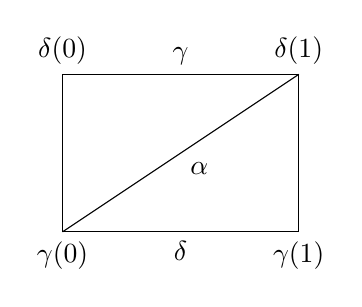
\begin{tikzpicture}
      \draw (0, 0) rectangle (3, 2);
      \draw (0, 0) -- (3, 2) node [pos=0.5, anchor=north west] {$\alpha$};
      \node [below] at (0, 0) {$\gamma(0)$};
      \node [below] at (3, 0) {$\gamma(1)$};
      \node [above] at (0, 2) {$\delta(0)$};
      \node [above] at (3, 2) {$\delta(1)$};

      \node [below] at (1.5, 0) {$\delta$};
      \node [above] at (1.5, 2) {$\gamma$};
    \end{tikzpicture}
  \end{center}
  Let $\alpha: [0, 1] \to X$ be a geodesic from $\gamma(0)$ to $\delta(1)$. Applying the CAT(0) estimate to $\Delta(\gamma(0), \gamma(1), \delta(1))$, we get
  \[
    d(\gamma(t), \alpha(t)) \leq d(\overline{\gamma(t)}, \overline{\alpha(t)}) = t d(\overline{\gamma(1)}, \overline{\alpha(1)}) = t d(\gamma(1), \alpha(1)) = t d(\gamma(1), \delta(1)),
  \]
  using what we know in plane Euclidean geometry. The same argument shows that
  \[
    d(\delta(t), \alpha(t) \leq (1 - t) d(\delta(0), \gamma(0)).
  \]
  So we know that
  \[
    d(\gamma(t), \delta(t)) \leq d(\gamma(t), \alpha(t)) + d(\alpha(t), \delta(t)) \leq (1 - t) d(\gamma(0), \delta(0)) + t d(\gamma(1), \delta(1)).
  \]
\end{proof}

\begin{lemma}
  If $X$ is CAT(0), then $X$ is \emph{uniquely geodesic}, i.e. each pair of points is joined by a unique geodesic.
\end{lemma}

\begin{proof}
  Suppose $x_0, x_1 \in X$ and $\gamma(0) = \delta(0) = x_0$ and $\gamma(1) = \delta(1) = x_1$. Then by the convexity of the metric, we have $d(\gamma(t), \delta(t)) \leq 0$. So $\gamma(t) = \delta(t)$ for all $t$. % Fix this proof. Do it directly.
\end{proof}
This is not surprising, because this is true in the Euclidean plane and the hyperbolic plane, but not in the sphere.

\begin{lemma}
  Let $X$ be a proper, uniquely geodesic metric space. Then geodesics in $X$ vary continuously with their end points in the compact-open topology (which is the same as the uniform convergence topology).
\end{lemma}
This is actually true without the word ``proper'', but the proof is harder

\begin{proof}
  This is an easy application of the Arzel\'a--Ascoli theorem.
\end{proof}

\begin{prop}
  Any proper CAT(0) space $X$ is contractible.
\end{prop}

\begin{proof}
  Pick a point $x_0 \in X$. Then the map $X \to \mathrm{Maps}([0, 1], X)$ sending $x$ to the unique geodesic from $x_0$ to $x$ is continuous. The adjoint map $X \times [0, 1] \to X$ is then a homotopy from the constant map at $x_0$ to the identity map.
\end{proof}

\begin{defi}[CAT(0) group]\index{CAT(0) group}
  A group is CAT(0) if it acts properly discontinuously and cocompactly by isometries on a proper CAT(0) space.
\end{defi}
Usually, for us, the action will also be free. This is the case, for example, when a fundamental group acts on the covering space.

\begin{eg}
  $\Z^n$ for any $n$ is CAT(0), since it acts on $\R^n$.
\end{eg}

\begin{eg}
  More generally, $\pi_1 M$ for any closed manifold $M$ of non-positive curvature is CAT(0).
\end{eg}

\begin{eg}
  Uniform lattices in semi-simple Lie groups. Examples include $\SL_n \mathcal{O}_K$ for certain number fields $K$.
\end{eg}
\begin{eg}
  Any free group, or direct product of free groups is CAT(0).
\end{eg}

We remark
\begin{prop}
  Any CAT(0) group $\Gamma$ satisfies a quadratic isoperimetric inequality, that is $\delta_\Gamma \simeq n$ or $\sim n^2$.
\end{prop}
We will not prove it.

Note that if $\Gamma$ is in fact CAT(-1), then $\Gamma$ is hyperbolic, which is not terribly difficult to see, since $\H^2$ is hyperbolic. But if a group is hyperbolic, is it necessarily CAT(-1)? Or even just CAT(0)? This is an open question. The difficulty in answering this question is that hyperbolicity is a ``coarse condition'', but being CAT(0) is a fine condition. For example, Cayley graphs are not CAT(0) spaces unless they are trees.

\subsection{Length metrics}
In differential geometry, if we have a covering space $\tilde{X} \to X$, and we have a Riemannian metric on $X$, then we can lift this to a Riemannian metric to $\tilde{X}$. This is possible since the Riemannian metric is a purely local notion, and hence we can lift it locally. Can we do the same for metric spaces?

Recall that if $\gamma: [a, b] \to X$ is a path, then
\[
  \ell(\gamma) = \sup_{a = t_0 < t_1 < \cdots < t_n = b} \sum_{i = 1}^n d(\gamma(t_{i - 1}), \gamma(t_i)).
\]
We say $\gamma$ is \emph{rectifiable} if $\ell(\gamma) < \infty$.

\begin{defi}[Length space]\index{length space}
  A metric space $X$ is called a \emph{length space} if for all $x, y \in X$, we have
  \[
    d(x, y) = \inf_{\gamma: x \to y} \ell(\gamma).
  \]
\end{defi}
Given any metric space $(X, d)$, we can construct a \term{length pseudometric} $\hat{d}: X \times X \to [0, \infty]$ given by
\[
  \hat{d}(x, y) = \inf_{\gamma: x \to y} \ell(\gamma).
\]
Now given a covering space $p: \tilde{X} \to X$ and $(X, d)$ a metric space, we can define a length pseudometric on $\tilde{X}$ by, for any path $\tilde{\gamma}: [a, b] \to \tilde{X}$,
\[
  \ell(\tilde{\gamma}) = \ell(p \circ \tilde{\gamma}).
\]
This induces an induced pseudometric on $\tilde{X}$.

\begin{ex}
  If $X$ is a length space, then so is $\tilde{X}$.
\end{ex}

Note that if $A, B$ are length spaces, and $X = A \cup B$ (such that the metrics agree on the intersection), then $X$ has a natural induced length metric. Recall we previously stated the Hopf--Rinow theorem in the context of differential geometry. In fact, it is actually just a statement about length spaces.

\begin{thm}[Hopf--Rinow theorem]\index{Hopf--Rinow theorem}
  If a length space $X$ is complete and locally compact, then $X$ is proper and geodesic.
\end{thm}
This is another application of the Arzel\'a--Ascoli theorem.

\subsection{Alexandrov's lemma}
Alexandrov's lemma is a lemma that enables us to glue CAT(0) space together to obtain new examples.

\begin{lemma}[Alexandrov's lemma]\index{Alexandrov's lemma}
  Suppose the triangles $\Delta_1 = \Delta(x, y, z_1)$ and $\Delta_2 = \Delta(x, y, z_2)$ in a metric space satisfy the CAT(0) condition, and $y \in [z_1, z_2]$.
  \begin{center}
    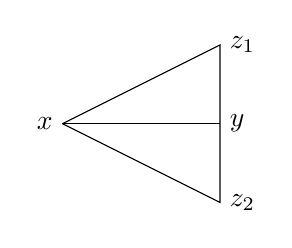
\begin{tikzpicture}
      \draw (0, 0) -- (2, 1) node [right] {$z_1$} -- (2, -1) node [right] {$z_2$} -- (0, 0) node [left] {$x$};
      \draw (0, 0) -- (2, 0) node [right] {$y$};
    \end{tikzpicture}
  \end{center}
  Then $\Delta = \Delta(x, z_1, z_2)$ also satisfies the CAT(0) condition.
\end{lemma}
This is the basic result we need if we want to prove ``gluing theorems'' for CAT(0) spaces.

\begin{proof}
  Consider $\bar{\Delta}_1$ and $\bar{\Delta}_2$, which together form a Euclidean quadrilateral $\bar{Q}$ with with vertices $\bra{x}, \bar{z}_1, \bar{z}_2, \bar{y}$. We claim that then the interior angle at $\bar{y}$ is $\geq 180^\circ$. Suppose not, and it looked like this:
  \begin{center}
    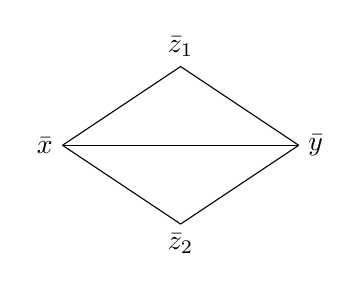
\begin{tikzpicture}
      \draw (0, 0) node [left] {$\bar{x}$} -- (3, 0) node [right] {$\bar{y}$};
      \draw (0, 0) -- (1.5, 1) node [above] {$\bar{z}_1$} -- (3, 0);
      \draw (0, 0) -- (1.5, -1) node [below] {$\bar{z}_2$} -- (3, 0);
    \end{tikzpicture}
  \end{center}
  If not, there exists $\bar{p}_i \in [\bar{y}, \bar{z}_i]$ such that $[\bar{p}_1, \bar{p}_2] \cap [\bar{x}, \bar{y}] = \{\bar{q}\}$ and $\bar{q} \not= \bar{y}$. Now
  \begin{align*}
    d(p_1, p_2) &= d(p_2, y) + d(y, p_2) \\
    &= d(\bar{p}_1, \bar{y}) + d(\bar{y}, \bar{p}_1)\\
    &= d(\bar{p}, \bar{y}) + d(\bar{y}, \bar{p}_2)\\
    &> d(\bar{p}_1, \bar{q}) + d(\bar{q}, \bar{p}_2)\\
    &\geq d(p_1, q) + d(q, p_2)\\
    &\geq d(p_1, p_2),
  \end{align*}
  which is a contradiction.

  Thus, we know the right picture looks like this:
  \begin{center}
    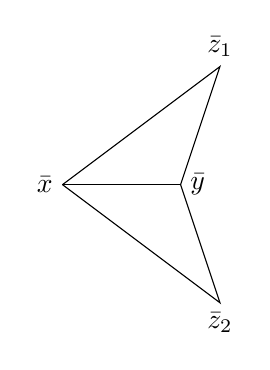
\begin{tikzpicture}
      \draw (0, 0) node [left] {$\bar{x}$} -- (1.5, 0) node [right] {$\bar{y}$};
      \draw (0, 0) -- (2, 1.5) node [above] {$\bar{z}_1$} -- (1.5, 0);
      \draw (0, 0) -- (2, -1.5) node [below] {$\bar{z}_2$} -- (1.5, 0);
    \end{tikzpicture}
  \end{center}
  To obtain $\bar{\Delta}$, we have to ``push'' $\bar{y}$ out so that the edge $\bar{z}_1 \bar{z}_2$ is straight, while keeping the lengths fixed. There is a natural map $\pi: \bar{\Delta} \to \bar{Q}$, and the lemma follows by checking that for any $a, b \in \bar{\Delta}$, we have
  \[
    d(\pi(a), \pi(b)) \leq d(a, b).
  \]
  This is an easy case analysis (or is obvious).
\end{proof}

A sample application is the following:
\begin{prop}
  If $X_1, X_2$ are both locally compact, complete CAT(0) spaces and $Y$ is isometric to closed, subspaces of both $X_1$ and $X_2$. Then $X_1 \cup_Y X_2$, equipped with the induced length metric, is CAT(0).
\end{prop}
\subsection{Cartan--Hadamard theorem}

\begin{thm}[Cartan--Hadamard theorem]\index{Cartan--Hadamard theorem}
  If $X$ is a complete, connected length space of non-positive curvature, then the universal cover $\tilde{X}$, equipped with the induced length metric, is CAT(0).
\end{thm}
This was proved by Cartan and Hadamard in the differential geometric setting.

\begin{cor}
  A (torsion free) group $\Gamma$ is CAT(0) iff it is the $\pi_1$ of a complete, connected space $X$ of non-positive curvature.
\end{cor}

We'll indicate some steps in the proof of the theorem.
\begin{lemma}
  If $X$ is proper, non-positively curved and uniquely geodesic, then $X$ is CAT(0).
\end{lemma}

\begin{proof}[Proof idea]
  The idea is that given a triangle, we cut it up into a lot of small triangles, and since $X$ is locally CAT(0), we can use Alexandrov's lemma to conclude that the large triangle is CAT(0).

  Recall that geodesics vary continuously with their endpoints. Consider a triangle $\Delta = \Delta (x, y, z) \subseteq \bar{B} \subseteq X$, where $\bar{B}$ is a compact ball. By compactness, there is an $\varepsilon$ such that for every $x \in \bar{B}$, the ball $B_x(\bar{\varepsilon})$ is CAT(0).

  We let $\beta_t$ be the geodesic from $x$ to $\alpha(t)$. Using continuity, we can choose $0 < t_1 < \cdots < t_N = 1$ such that
  \[
    d(\beta_{t_i}(s), \beta_{t_{i + 1}}(s)) < \varepsilon
  \]
  for all $s \in [0, 1]$.

  Now divide $\Delta$ up into a ``patchwork'' of triangles, each contained in an $\varepsilon$ ball, so each satisfies the CAT(0) condition, and apply induction and Alexandrov's lemma to conclude.
\end{proof}

Now to prove the Cartan--Hadamard theorem, we only have to show that the universal cover is uniquely geodesic. Here we must use the simply-connectedness condition.
\begin{thm}
  Let $X$ be a proper length space of non-positive curvature, and $p, q \in X$. Then each homotopy class of paths from $p$ to $q$ contains a \emph{unique} (local) geodesic representative.
\end{thm}

\subsection{Gromov's link condition}
Gromov's link condition is a criterion that makes it very easy to write down interesting examples of non-positively-curved metric spaces.

\begin{defi}[Euclidean cell complex]\index{Euclidean cell complex}
  A locally finite cell complex $X$ is \emph{Euclidean} if every cell is isometric to a convex polyhedron in Euclidean space and the attaching maps to identify faces isometrically with lower-dimensional cells.
\end{defi}
Such a complex $X$ has a natural length metric which is proper and geodesic by Hopf--Rinow. What we'd like to do is to come up with a condition that ensures $X$ is CAT(0).

\begin{eg}
  The usual diagram for a torus gives an example of a Euclidean complex.
  \begin{center}
    \begin{tikzpicture}
      \draw [->-=0.55, mred] (0, 0) -- (3, 0);
      \draw [->-=0.55, mred] (0, 3) -- (3, 3);

      \draw [->-=0.55, mblue] (0, 0) -- (0, 3);
      \draw [->-=0.55, mblue] (3, 0) -- (3, 3);
    \end{tikzpicture}
  \end{center}
\end{eg}

\begin{eg}
  We can construct a sphere this way, just by taking a cube!
\end{eg}
We know that $T^2$ is non-positively curved (since it is flat), but the cube is not, because by Cartan--Hadamard, it would be CAT(0), hence contractible, but it is not.

\begin{defi}[Link]\index{link}
  Let $X$ be a Euclidean complex, and let $v$ be a vertex of $X$, and let $0 < \varepsilon \ll \text{shortest $1$-cell}$. Then the \emph{link} of $v$ is
  \[
    Lk(v) = S_v(\varepsilon) = \{x \in X: d(x, v) = \varepsilon\}.
  \]
\end{defi}
Note that $Lk(V)$ is a cell complex: the intersection of $Lk(v)$ with a cell of $X$ of dimension is a cell of dimension $n - 1$.

\begin{eg}
  In the torus, there is only one vertex. The link looks like
  \begin{center}
    \begin{tikzpicture}
      \draw [->-=0.55, mred] (0, 0) -- (3, 0);
      \draw [->-=0.55, mred] (0, 3) -- (3, 3);

      \draw [->-=0.55, mblue] (0, 0) -- (0, 3);
      \draw [->-=0.55, mblue] (3, 0) -- (3, 3);

      \draw (0, 0.3) arc(90:0:0.3);
      \draw (3, 0.3) arc(90:180:0.3);
      \draw (0, -0.3) arc(-90:0:0.3);
      \draw (3, -0.3) arc(-90:-180:0.3);
    \end{tikzpicture}
  \end{center}
  So the link is $S^1$.
\end{eg}

\begin{eg}
  If we take the corner of a cube, then $Lk(v)$ is homeomorphic to $S^1$, but it is a weird one, because it is made up of three right angles, not two.
\end{eg}

How can we distinguish between these two $S^1$'s? \emph{Angle} puts a metric on $Lk(v)$. We can do this for general metric spaces, but we only need it for Euclidean complexes, in which case there is not much to do.

Restricted to each cell, the link is just a part of a sphere, and it has a natural spherical metric, which is a length metric. These then glue together to a length metric on $Lk(v)$. Note that this is not the same as the induced metric.

\begin{eg}
  In the torus, the total length of the link is $2\pi$, while that of the cube is $\frac{3\pi}{2}$.
\end{eg}

\begin{thm}[Gromov's link criterion]\index{Gromov's link criterion}
  A Euclidean complex $X$ is non-positively-curved iff for every vertex $v$ of $X$, $Lk(v)$ is CAT(1).
\end{thm}
Note that by definition, we only have to check the CAT(1) inequality on triangles of perimeter $< 2\pi$.

\begin{ex}
  Check these in the case of the torus and the cube.
\end{ex}

Thus, given a group, we can try to construct a space whose $\pi_1$ is it, and then put a Euclidean structure on it, then check Gromov's link criterion.

In general, Gromov's link condition might not be too useful, because we still don't know how to check if something is CAT(1)! However, it is very simple in dimension $2$.

\begin{cor}
  If $X$ is a $2$-dimensional Euclidean complex, then for all vertices $v$, $Lk(v)$ is a metric graph, and $X$ is CAT(0) iff $Lk(v)$ has no loop of length $< 2\pi$ for all $v$.
\end{cor}

\begin{eg}[Wise's example]\index{Wise's example}
  Consider the group
  \[
    W = \bra a, b, s, t \mid [a, b] = 1, s^{-1}as = (ab)^2, t^{-1}bt = (ab)^2\ket.
  \]
  Letting $c = ab$, it is easy to see that this is the $\pi_1$ of the following Euclidean complex:
  \begin{center}
    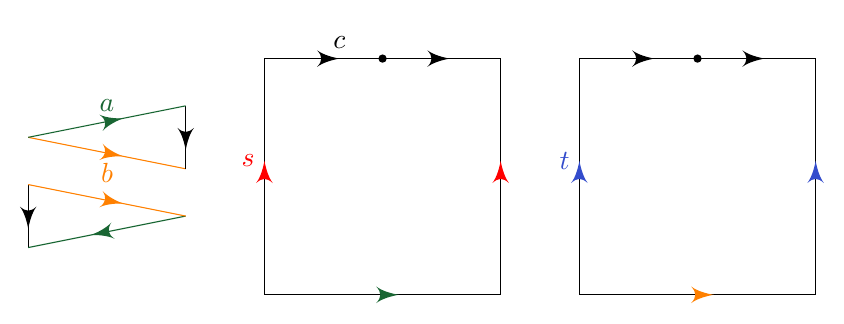
\begin{tikzpicture}
      \begin{scope}[ xscale=2]
        \draw [->-=0.6, morange] (0, 0.5) -- (1, 0.1) node [pos=0.5, below] {$b$};
        \draw [-<-=0.3] (1, 0.1) -- (1, 0.9);
        \draw [-<-=0.4, mgreen] (1, 0.9) -- (0, 0.5) node [pos=0.5, above] {$a$};

        \draw [->-=0.7] (0, -0.1) -- (0, -0.9);
        \draw [-<-=0.4, mgreen] (0, -0.9) -- (1, -0.5);
        \draw [-<-=0.4, morange] (1, -0.5) -- (0, -0.1);% two purple vertices, one red vertex
      \end{scope}

      \draw (3, 1.5) rectangle (6, -1.5); % blue right angles
      \draw (7, 1.5) rectangle (10, -1.5);

      \node [circ] at (4.5, 1.5) {};
      \node [circ] at (8.5, 1.5) {};

      \draw [->] (3.95, 1.5) -- +(0.0001, 0) node [above] {$c$};
      \draw [->] (5.35, 1.5) -- +(0.0001, 0);

      \draw [->] (7.95, 1.5) -- +(0.0001, 0);
      \draw [->] (9.35, 1.5) -- +(0.0001, 0);

      \draw [->, mgreen] (4.7, -1.5) -- +(0.0001, 0);
      \draw [->, morange] (8.7, -1.5) -- +(0.0001, 0);

      \draw [->, red] (3, 0.2) -- +(0, 0.0001) node [left] {$s$};
      \draw [->, red] (6, 0.2) -- +(0, 0.0001);
      \draw [->, mblue] (7, 0.2) -- +(0, 0.0001) node [left] {$t$};
      \draw [->, mblue] (10, 0.2) -- +(0, 0.0001);
    \end{tikzpicture}
  \end{center}
  This is metrized in the obvious way, where all edges have length $2$ except the black ones of length $1$. To understand the links, we set
  \[
    \alpha = \sin^{-1}\frac{1}{4},\quad \beta = \cos^{-1} \frac{1}{4}.
  \]
  Then the triangles each has angles $2\alpha, \beta, \beta$.

  We show that $W$ is non-positively curved, and then use this to show that there is a homomorphism $W \to W$ that is surjective but not injective. We say $W$ is \term{non-Hopfian}. In particular, this will show that $WW$ is not linear, i.e.\ it is not a matrix group.

  To show that $X$ is non-positively curved, we check the link condition:
  \begin{center}
    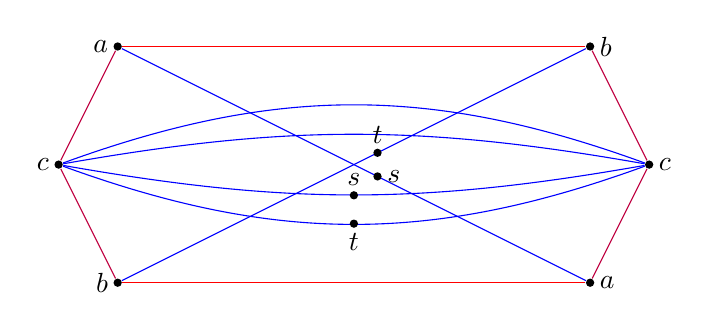
\begin{tikzpicture}[scale=1.5]
      \node [circ] at (-2.5, 0) (left) {};
      \node [circ] at (-2, 1) (topleft) {};
      \node [circ] at (-2, -1) (bottomleft) {};
      \node [circ] at (2.5, 0) (right) {};
      \node [circ] at (2, 1) (topright) {};
      \node [circ] at (2, -1) (bottomright) {};

      \node [left] at (topleft) {$a$};
      \node [right] at (bottomright) {$a$};
      \node [left] at (left) {$c$};
      \node [right] at (right) {$c$};
      \node [left] at (bottomleft) {$b$};
      \node [right] at (topright) {$b$};

      \draw [red] (topleft) -- (topright);
      \draw [red] (bottomleft) -- (bottomright);
      \draw [purple] (bottomleft) -- (left) -- (topleft);
      \draw [purple] (bottomright) -- (right) -- (topright);

      \draw [blue] (bottomleft) -- (topright);
      \draw [blue] (topleft) -- (bottomright);
      \draw [blue] (left) edge [bend left=10] (right);
      \draw [blue] (left) edge [bend right=10] (right);
      \draw [blue] (left) edge [bend left=20] (right);
      \draw [blue] (left) edge [bend right=20] (right);

      \node [circ] at (0.2, 0.1) {};
      \node [circ] at (0.2, -0.1) {};

      \node [circ] at (0, -0.26) {};
      \node [circ] at (0, -0.5) {};
      \node [below] at (0, -0.5) {$t$};
      \node [above] at (0.2, 0.1) {$t$};
      \node [right] at (0.2, -0.1) {$s$};
      \node [above] at (0, -0.26) {$s$};

      % label intermediate nodes in blue thing as $s$ and $t$, each occurring twice
    \end{tikzpicture}
  \end{center}
  To check the link condition, we have to check that there are no loops of length $< 2\pi$ in $Lk(v)$. Note that by trigonometric identities, we know $\alpha + \beta = \frac{\pi}{2}$. So we can just observe that everything is fine.

  To see that $W$ is non-Hopfian, we define
  \begin{align*}
    f: W &\to W\\
    a &\mapsto a^2\\
    b &\mapsto b^2\\
    s &\mapsto s^2\\
    t &\mapsto t
  \end{align*}
  We check that this is a well-defined homomorphism, and is surjective, since we observe
  \[
    a = s a^2 b^2 s^{-1},\quad b = ta^2 b^2 t^{-1},
  \]
  and so $a, b, s, t \in \im t$. The non-trivial claim is that $\ker f \not 0$. Let
  \[
    g = [scs^{-1}, tct^{-1}].
  \]
  Note that
  \[
    f(g) = [f(scs^{-1}), f(tct^{-1})] = [sc^2 s^{-1}, tc^2 t^{-1}] = [a, b] = 1.
  \]
  So the crucial claim is that $g \not= 1$. This is where geometry comes to the rescue. For convenience, write $p = scs^{-1}, q = tct^{-1}$. Consider the following local geodesics in the two squares:
  \begin{center}
    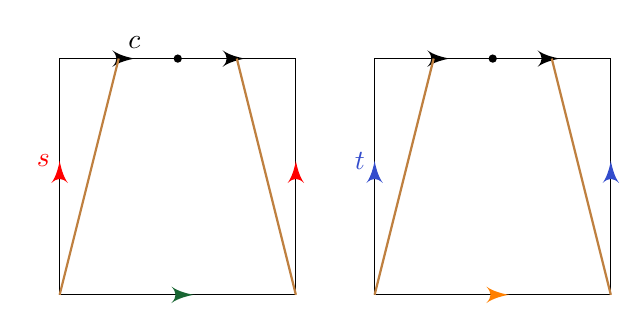
\begin{tikzpicture}
      \draw (3, 1.5) rectangle (6, -1.5);
      \draw (7, 1.5) rectangle (10, -1.5);

      \node [circ] at (4.5, 1.5) {};
      \node [circ] at (8.5, 1.5) {};

      \draw [->] (3.95, 1.5) -- +(0.0001, 0) node [above] {$c$};
      \draw [->] (5.35, 1.5) -- +(0.0001, 0);

      \draw [->] (7.95, 1.5) -- +(0.0001, 0);
      \draw [->] (9.35, 1.5) -- +(0.0001, 0);

      \draw [->, mgreen] (4.7, -1.5) -- +(0.0001, 0);
      \draw [->, morange] (8.7, -1.5) -- +(0.0001, 0);

      \draw [->, red] (3, 0.2) -- +(0, 0.0001) node [left] {$s$};
      \draw [->, red] (6, 0.2) -- +(0, 0.0001);
      \draw [->, mblue] (7, 0.2) -- +(0, 0.0001) node [left] {$t$};
      \draw [->, mblue] (10, 0.2) -- +(0, 0.0001);

      \draw [thick, brown] (3, -1.5) -- (3.75, 1.5);
      \draw [thick, brown] (5.25, 1.5) -- (6, -1.5);

      \draw [thick, brown] (7, -1.5) -- (7.75, 1.5);
      \draw [thick, brown] (9.25, 1.5) -- (10, -1.5);
    \end{tikzpicture}
  \end{center}
  The left- and right-hand local geodesics represent $p$ and $q$ respectively. Then
  \[
    g = p \cdot q \cdot \bar{p} \cdot \bar{q}.
  \]
  We claim that this represents $g$ by a local geodesic. The only place that can go wrong is the points where they are joined. By the proof of the Gromov link condition, to check this, we check that the three ``turns'' at the vertex are all of angle $\geq \pi$.
  \begin{center}
    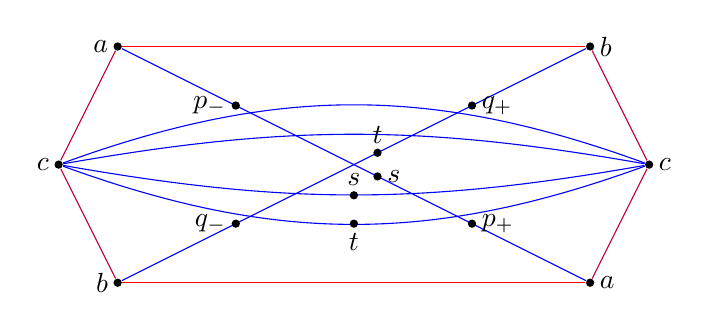
\begin{tikzpicture}[scale=1.5]
      \node [circ] at (-2.5, 0) (left) {};
      \node [circ] at (-2, 1) (topleft) {};
      \node [circ] at (-2, -1) (bottomleft) {};
      \node [circ] at (2.5, 0) (right) {};
      \node [circ] at (2, 1) (topright) {};
      \node [circ] at (2, -1) (bottomright) {};

      \node [left] at (topleft) {$a$};
      \node [right] at (bottomright) {$a$};
      \node [left] at (left) {$c$};
      \node [right] at (right) {$c$};
      \node [left] at (bottomleft) {$b$};
      \node [right] at (topright) {$b$};

      \draw [red] (topleft) -- (topright);
      \draw [red] (bottomleft) -- (bottomright);
      \draw [purple] (bottomleft) -- (left) -- (topleft);
      \draw [purple] (bottomright) -- (right) -- (topright);

      \draw [blue] (bottomleft) -- (topright);
      \draw [blue] (topleft) -- (bottomright);
      \draw [blue] (left) edge [bend left=10] (right);
      \draw [blue] (left) edge [bend right=10] (right);
      \draw [blue] (left) edge [bend left=20] (right);
      \draw [blue] (left) edge [bend right=20] (right);

      \node [circ] at (0.2, 0.1) {};
      \node [circ] at (0.2, -0.1) {};

      \node [circ] at (0, -0.26) {};
      \node [circ] at (0, -0.5) {};
      \node [below] at (0, -0.5) {$t$};
      \node [above] at (0.2, 0.1) {$t$};
      \node [right] at (0.2, -0.1) {$s$};
      \node [above] at (0, -0.26) {$s$};

      \node [circ] at (-1, -0.5) {};
      \node [circ] at (1, -0.5) {};
      \node [circ] at (-1, 0.5) {};
      \node [circ] at (1, 0.5) {};

      \node [right] at (1, 0.5) {$q_+$};
      \node [left] at (-1, -0.5) {$q_-$};
      \node [left] at (-1, 0.5) {$p_-$};
      \node [right] at (1, -0.5) {$p_+$};
    \end{tikzpicture}
  \end{center}
  Here $p_+$ is the point where $p$ ends and $p_-$ is the point where $p$ starts, and similarly for $q$. Moreover, the distance from $p_{\pm}, q_{\pm}$ to the top/bottom left/right vertices is $\beta$. So we can just check and see that everything works.

  Recall that every homotopy class of paths in $X$ contains a \emph{unique} locally geodesic representative. Since the constant path is locally geodesic, we know $g \not= 1$.
\end{eg}

\begin{defi}[Residually finite group]\index{residually finite group}
  A group $G$ is \emph{residually finite} if for every $g \in G \setminus \{1\}$, there is a homomorphism $\varphi: G \to \text{finite group}$ such that $\varphi(g) \not= 0$.
\end{defi}

\begin{thm}[Mal'cev]
  Every finitely generated linear subgroup (i.e.\ a subgroup of $\GL_n(\C)$) is resudially finite.
\end{thm}

\begin{proof}[Proof sketch]
  If the group is in fact a subgroup of $\GL_n(\Z)$, then we just reduce mod $p$ for $p \gg 0$. To make it work over $\GL_n(\C)$, we need a suitable version of the Nullstellensatz.
\end{proof}

\begin{thm}[Mal'cev]
  Every finitely generated residually finite group is Hopfian.
\end{thm}

\begin{proof}
  Finding a proof is a fun exercise!
\end{proof}
We know that Wise's example is not Hopfian, hence not residually finite, hence not a linear group.

Contrast this with the amazing theorem of Sela that all hyperbolic groups are Hopfian. However, a major open question is whether all hyperbolic groups are residually finite. On the other hand, it is known that not all hyperbolic groups are not linear.

How are we supposed to think about residually finite groups?

\begin{lemma}[Scott's criterion]\index{Scott's criterion}
  Let $X$ be a cell complex, and $G = \pi_1 X$. Then $G$ is residually finite if and only if the following holds:

  Let $p: \tilde{X} \to X$ be the universal cover. For all compact subcomplexes $K \subseteq \tilde{X}$, there is a finite-sheeted cover $X' \to X$ such that the natural covering map $p': \tilde{X} \to X'$ is injective on $K$.
\end{lemma}
A good (though not technically correct) way to think about this is follows: if we have a map $f: K \to X$ that may be complicated, and in particular is not injective, then we might hope that there is some ``finite resolution'' $X' \to X$ such that $f$ lifts to $X'$, and the lift is injective. Of course, this is not always possible, and a necessary condition for this to work is that the lift to the universal cover is injective. If this is not true, then obviously no such resolution can exist. And residual finiteness says if there is not obvious reason to fail, then it in fact does not fail.

\subsection{Cube complexes}
\begin{defi}[Cube complex]\index{cube complex}
  A Euclidean complex is a \emph{cube complex} if every cell is isometric to a cube (of any dimension).
\end{defi}
This is less general than Euclidean complexes, but we can still make high dimension things out of this. Of course, general Euclidean complexes also work in high dimensions, but except in two dimensions, the link condition is rather tricky to check in higher dimensional situations. It turns out the link condition is easy to check for cube complexes.

Purely topologically, the link of each vertex is made out of simplices, and, subdividing if necessary, they are simplicial complexes. The metric is such that every edge has length $\frac{\pi}{2}$, and this is called the ``all-right simplicial complex''.

Recall that
\begin{center}
  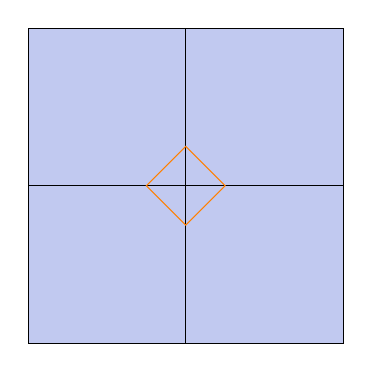
\begin{tikzpicture}
    \draw [fill=mblue, fill opacity=0.3] (-2, -2) rectangle (2, 2);
    \draw (0, -2) -- (0, 2);
    \draw (-2, 0) -- (2, 0);
    \draw [morange] (0.5, 0) -- (0, 0.5) -- (-0.5, 0) -- (0, -0.5) -- cycle;
  \end{tikzpicture}
\end{center}
is non-positively curved, while
\begin{center}
  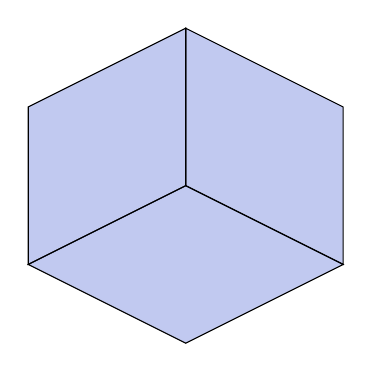
\begin{tikzpicture}
    \draw [fill=mblue, fill opacity=0.3] (0, 0) -- (0, 2) --(2, 1) -- (2, -1) -- cycle;
    \draw [fill=mblue, fill opacity=0.3] (0, 0) -- (0, 2) --(-2, 1) -- (-2, -1) -- cycle;

    \draw [fill=mblue, fill opacity=0.3] (2, -1) -- (0, 0) -- (-2, -1) -- (0, -2) -- cycle; % draw triangle
  \end{tikzpicture}
\end{center}
is not.

\begin{defi}[Flag simplicial complex]\index{flag simplicial complex}
  A simplicial complex is not \emph{flag} if for some $n \geq 2$, it contains a $1$-dimensional subcomplex isomorphic to the $1$-skeleton of an $n$-simplex, which is not contained in the boundary of an $n$-simplex.

  A flag simplicial complex is one that is not not flag.
\end{defi}
So we cannot contain an empty triangle, or hollow tetrahedra.

Note that topologically, flag complexes are not special in any sense. For any simplicial complex $K$, the first barycentric subdivision is flag.

\begin{thm}[Gromov]
  A cube complex is non-positively curved iff every link is flag.
\end{thm}
Now the property of being flag is purely combinatorial, and easy to check. So this lets us work with cube complexes.

\subsubsection*{Right-angled Artin groups}
\begin{defi}[right-angled Artin group]\index{right-angled Artin group}
  Let $N$ be a simplicial graph, i.e.\ a graph where the vertices determine the edges, i.e.\ a graph as a graph theorist would consider. Then
  \[
    A_N = \bra V(N) \mid [u, v] = 1 \text{ for all } (u, v) \in E(N)\ket
  \]
  is the \emph{right-angled Artin group}, or \term{graph group}.
\end{defi}

\begin{eg}
  If $N$ is the discrete graph on $n$ vertices, then $A_N = F_n$.
\end{eg}

\begin{eg}
  If $N$ is the complete graph on $n$ vertices, then $A_N = \Z^n$.
\end{eg}

\begin{eg}
  If $N$ is a square, i.e.\ the complete bipartite graph $K_{2, 2}$, then $A_N = F_2 \times F_2$.
\end{eg}

\begin{eg}
  When $N$ is the path with $4$ vertices, then this is a complicated group that doesn't have a good, alternative description. This is quite an interesting group.
\end{eg}

\begin{defi}[Salvetti complex]\index{Salvetti complex}
  $\mathcal{S}_N$ is a cube complex defined as follows:
  \begin{itemize}
    \item Set $\mathcal{S}_N^{(2)}$ is the presentation complex for $A_N$.
    \item For any immersion of the $2$-skeleton of a $d$-dimensional cube, we glue in an $d$-dimensional cube to $\mathcal{S}_N^{(2)}$.
  \end{itemize}
  Alternatively, we have a natural inclusion $\mathcal{S}_N^{(2)} \subseteq (S^1)^{|V(N)|}$, and $\mathcal{S}_N$ is the largest subcomplex whose $2$-skeleton coincides with $\mathcal{S}_N^{(2)}$.
\end{defi}

\begin{eg}
  If $N$ is
  \begin{center}
    \begin{tikzpicture}
      \node [circ] at (0, 0) {};
      \node [circ] at (1, 0) {};
      \node [circ] at (2, 0) {};
      \draw (1, 0) -- (2, 0);
    \end{tikzpicture}
  \end{center}
  then $A_n = \Z * \Z^2$, and $\mathcal{S}_N$ is a circle glued to a torus.
\end{eg}

\begin{defi}[Flag complex]\index{flag complex}
  The \emph{flag complex} of $N$, written $\bar{N}$, is the only flag simplicial complex with $1$-skeleton $N$.
\end{defi}

\begin{eg}
  If $N$ is
  \begin{center}
    \begin{tikzpicture}
      \node [circ] at (0, 0) {};
      \node [circ] at (1, 0) {};
      \node [circ] at (2, 0) {};
      \draw (0, 0) -- (1, 0);
    \end{tikzpicture},
  \end{center}
  then $\mathcal{S}_N$ is $T^2 \vee S^1$. There is a unique vertex $v$, and its link looks like
  \begin{center}
    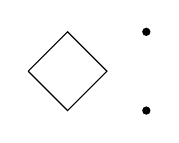
\begin{tikzpicture}
      \draw (-0.5, 0) -- (0, 0.5) -- (0.5, 0) -- (0, -0.5) -- (-0.5, 0);

      \node [circ] at (1, 0.5) {};
      \node [circ] at (1, -0.5) {};
    \end{tikzpicture}
  \end{center}
\end{eg}
In fact, there is a recipe for getting the link out of $N$.

\begin{defi}[Double]\index{double}\index{$D(K)$}
  the \emph{double} $D(K)$ of a simplicial complex $K$ is defined as follows:
  \begin{itemize}
    \item The vertices are $\{v_1^+, \ldots, v_n^+, v_1^-, \ldots, v_n^-\}$, where $\{v_1, \ldots, v_n\}$ are the vertices of $k$.
    \item The simplices are those of the form $\bra v_{i_0}^{\pm}, \ldots, v_{i_k}^{\pm}\ket$, where $\bra v_{i_0}, \ldots, v_{i_k}\ket \in K$.
  \end{itemize}
\end{defi}

\begin{eg}
  The double of $N$ is just $Lk(v)$!
\end{eg}

Note that $D(K)$ contains many copies of $K$, especially $K^+$, which is spanned by the $v_i^+$, and $K^-$, which is spanned by the $v_i^-$. In fact, $K^+$ (and also $K^-$) is a retract of $D(K)$, using the map that sends $v^{\pm}_i$ to $v_i$. Note also that $D(K)$ is flag iff $K$ is flag.

\begin{lemma}
  For any (simplicial) graph $N$, the link of the unique vertex of $\mathcal{S}_N$ is $D(\bar{N})$. In particular, $\mathcal{S}_N$ is non-positively curved.
\end{lemma}

Thus, right-angled Artin groups and their Salvetti complexes give examples of non-positively curved spaces with very general links. It turns out

\begin{thm}
  Right-angled Artin groups embed into $\GL_n\Z$ (where $n$ depends on $N$).
\end{thm}

\subsection{Special cube complexes}
Let $X$ be a non-positively curved cube complex. We will write down explicit geometric/combinatorial conditions on $X$ so that $\pi_1 X$ embeds into $A_N$ for some $N$.

\subsubsection*{Hyperplanes and their pathologies}
If $C \cong [-1, 1]^n$, then a \term{midcube} $M \subseteq C$ is the intersection of $C$ with $\{x_i = 0\}$ for some $i$.

% insert picture

Now if $X$ is a non-positively curved cube complex, and $M_1, M_2$ are midcubes of cubes in $X$, we say $M_1 \sim M_2$ if they have a common face, and extend this to an equivalence relation. The equivalence classes are \emph{immersed hyperplanes}. We usually visualize these as the union of all the midcubes in the equivalence class.

An immersed hyperplane can be thought of as a locally isometric map $H \looparrowright X$, where $H$ is a cube complex. Let $N_H$ be the pullback interval bundle over $H$. That is, $N_H$ Is obtained by gluing together $\{M \times (-1, 1) \mid M\text{ is a cube in }H\}$. The point of this is to resolve the self-intersections.

% insert picture

% insert M\"obius band example.

$N_H$ is always a $(-1, 1)$-bundle over $H$, and this corresponds to a homomorphism $\pi_1 H \to \Isom(-1, 1) \cong \Z/2$. If this homomorphism is trivial, then we say $H$ is \term{two-sided}. Otherwise, $H$ is \term{one-sided}.

We have now met two pathologies of hyperplanes: they may be one-sided (e.g.\ a M\"obius band), or have self-intersections. There are two more. The first is \term{self osculations}:

% insert pictures

Note that it makes sense to distinguish between direct and indirect osculations only if our hyperplane is two-sided.

Finally, we have \term{inter-osculations}:

% another picture

\begin{defi}[Special cube complex (Haglund--Wise)]\index{special cube complex}\index{cube complex!special}
  A cube complex is \emph{special} if its hyperplanes do not exhibit any of the following four pathologies:
  \begin{itemize}
    \item One-sidedness
    \item Self-intersection
    \item Direct self-osculation
    \item Inter-osculation
  \end{itemize}
\end{defi}

\begin{eg}
  A cube is a special cube complex.
\end{eg}

\begin{eg}
  Traditionally, the way to exhibit a surface as a cube complex is to first tile it by right-angled polygons, so that every vertex has degree $4$, and then the dual exhibits the surface as a cube complex. The advantage of this approach is that the hyperplanes are exactly the edges in the original tiling!

  % insert picture

  From this, one checks that we in fact have a special curve complex.
\end{eg}
This is one example, but it is quite nice to have infinitely many. It is true that covers of special things are special. So this already gives us infinitely many special cube complexes. But we want others.

\begin{eg}
  If $X = \mathcal{S}_N$ is a Salvetti complex, then it is a special cube complex, and it is not terribly difficult to check.
\end{eg}

\begin{thm}[Haglund--Wise]
  If $X$ is a compact special cube complex, then there exists a graph $N$ and a local isometry of cube complexes
  \[
    \varphi_X: X \looparrowright \mathcal{S}_N.
  \]
\end{thm}

\begin{cor}
  $\pi_1 X \hookrightarrow A_N$.
\end{cor}

\begin{proof}
  If $g \in \pi_1 X$, then $g$ is uniquely represented by a local geodesic $\gamma: I \to X$. Then $\varphi \circ \gamma$ is a local geodesic in $\mathcal{S}_N$. Since homotopy classes of loops are represented by unique local geodesics, this implies $\varphi_X \circ \gamma$ is not null-homotopic. So the map $(\varphi_X)_*$ is injective.
\end{proof}

So if we know some nice group-theoretic facts about right-angled Artin groups, then we can use them to understand $\pi_1X$. For example,
\begin{cor}
  If $X$ is a special cube complex, then $\pi_1 X$ is linear, residually finite, Hopfian, etc.
\end{cor}
We shall try to give an indication of how we can prove the Haglund--Wise theorem. We first make the following definition.
\begin{defi}[Virtually special group]\index{virtually special proof}
  A group $\Gamma$ is \emph{virtually special} if there exists a finite index subgroup $\Gamma_0 \leq \Gamma$ such that $\Gamma_0 \cong \pi_1 X$, where $X$ is a compact special cube complex.
\end{defi}

\begin{proof}[Sketch proof of Haglund--Wise]
  We have to first come up with an $N$. We set the vertices of $N$ to be the hyperplanes of $X$, and we join two vertices iff the hyperplanes cross in $X$. This gives $\mathcal{S}_N$. We choose a transverse orientation on each hyperplane of $X$.

  Now we define $\varphi_X: X \looparrowright \mathcal{S}_N$ cell by cell.
  \begin{itemize}
    \item Vertices: There is only one vertex in $\mathcal{S}_N$.
    \item Edges: Let $e$ be an edge of $X$. Then $e$ crosses a unique hyperplane $H$. Then $H$ is a vertex of $N$. This corresponds to a generator in $A_N$, hence a corresponding edge $e(H)$ of $\mathcal{S}_N$. Send $e$ to $e(H)$. The choice of transverse orientation tells us which way round to do it
    \item Squares: given a hyperplane
      \begin{center}
        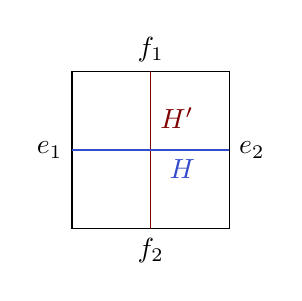
\begin{tikzpicture}
          \draw (0, 0) -- (2, 0) node [below, pos=0.5] {$f_2$} -- (2, 2) node [right, pos=0.5] {$e_2$} -- (0, 2) node [pos=0.5, above] {$f_1$} -- (0, 0) node [pos=0.5, left] {$e_1$};

          \draw [mred] (1, 0) -- (1, 2) node [pos=0.7, right] {$H'$};
          \draw [mblue] (0, 1) -- (2, 1) node [pos=0.7, below] {$H$};
        \end{tikzpicture}
      \end{center}
      Note that we already mapped $e_1, e_2$ to $e(H)$, and $f_1, f_2$ to $e(H')$. Since $H$ and $H'$ cross in $X$, we know $e(H)$ and $e(H')$ bound a square in $\mathcal{S}_N$. Send this square in $X$ to that square in $\mathcal{S}_N$.
    \item There is nothing to do for the higher-dimensional cubes, since by definition of $\mathcal{S}_N$, they have all the higher-dimensional cubes we can hope for.
  \end{itemize}
  We haven't used a lot of the nice properties of special cube complexes. They are needed to show that the map is a local isometric embedding. What we do is to use the hypothesis to show that the induced map on links is an isometric embedding, which implies $\varphi_X$ Is a local isometry.
\end{proof}

This really applies to a really wide selection of objects.
\begin{eg}
  The following groups are virtually special groups:
  \begin{itemize}
    \item $\pi_1 M$ for $M$ almost any $3$-manifold.
    \item Random groups
  \end{itemize}
\end{eg}
This is pretty amazing. A ``random group'' is linear!
\printindex
\end{document}
